\documentclass[3p,sort&compress]{elsarticle}
\usepackage[USenglish]{babel}
\usepackage{amsmath}
\usepackage{amssymb}
\usepackage{ragged2e}
\usepackage{amsthm}
\usepackage{MnSymbol}
\usepackage{bbm}
\usepackage[titletoc,toc,title]{appendix}
\usepackage{natbib}
\usepackage{subfig}
\usepackage{graphicx}
\usepackage{siunitx}
\usepackage{lineno}
\usepackage{hyperref}
\usepackage{todonotes}
\usepackage{proba}
\usepackage{cleveref}
\usepackage{booktabs}
\usepackage{subfig}
\newtheorem{definition}{Definition}
\newtheorem{theorem}{Theorem}[section]
\newtheorem{corollary}{Corollary}%[theorem]
\newtheorem{lemma}[theorem]{Lemma}
\newtheorem*{remark}{Remark}
\newtheorem{assumption}{Assumption}
\providecommand{\abs}[1]{\lvert#1\rvert}
\providecommand{\norm}[1]{\lVert#1\rVert}
\DeclareRobustCommand{\1}[1]{\ensuremath \mathbbm{1}_{\{#1\}}}
\journal{Physica A}
%%%%%%%%%%%%%%%%%%%%%%%%%%%%%%%%%%%%%%%%%%%%%%%%%%%%%%%%%%%
\modulolinenumbers[1]
\begin{document}
	\begin{frontmatter}
		\title{
			Stochastic Asymptotic 
			Analysis  of a Multi-Host 
			Model with Vector Transmission.
		}
		\tnotetext[mytitlenote]{
			Departamento de Matem\'aticas, divisi\'on de Posgrado.
		}
		\author{Manuel Adrian Acu\~na-Zegarra\fnref{myfootnote}}
		\address{Radarweg 29, Amsterdam}
		\fntext[myfootnote]{Since 1880.}
%
		\author[mymainaddress,mysecondaryaddress]{Sa\'ul D\'iaz-Infante}
		\ead[url]{www.elsevier.com}
		\author[mysecondaryaddress]%
		{Daniel Olmos-Liceaga \corref{mycorrespondingauthor}}
		\cortext[mycorrespondingauthor]{Corresponding author}
		\ead{saul.diazinfante@unison.mx}
		\address[mymainaddress]{Universidad de Sonora, Hermosillo, Sonora, M\'exico}
		\address[mysecondaryaddress]{360 Park Avenue South, New York}
		\begin{abstract}
				We present a stochastic extension of a disease vector transmission model with 
multi-hosts. Our deterministic dynamics considers vectors and his interacting 
with two kind of hosts. Applying a general stochastic perturbation 
to a vector biting rate, we extend to a stochastic differential 
equation system (SDEs), which model the influence of environmental noise on the 
vector transmission. 
		\end{abstract}
		\begin{keyword}
			Multi-host, persistence, extinction, stochastic perturbation,
			vector transmission.
		\end{keyword}
	\end{frontmatter}
	\linenumbers
	\section{Introduction}
		\paragraph{Motivation}
	Now days, vector diseases represents the principal cause of death in 
many sub development countries. A combination of low resources, climate
variations and lack of efficient health services, amplifies its prevalence. So, 
design tools to planing strategies under real conditions is crucial. However
this phenomena depends on many and very intricate variables. 
By this reason, not exist a general model which  describe or predict in a
acceptable way, the essence of this complex system. Instead, a lot of literature
focus on describe a specific characteristic under restrictive or unrealistic 
conditions. We believe that to incorporate uncertainty is an clever option
~--- resume the effect of many variables as "noise" ~---to produce a more 
realistic model.

	

\todo{Find other diseases, structure and use Chagas 
	like example, leismaniasis, peste (sin tratamiento).}
\paragraph{Previous and related work}
	Essentially, in literature exist two main alternatives 
	for incorporate environmental noise. The first alternative, considers as step 
	one, to describe the disease transitions with a discrete Markov chain. Next,
	letting discrete time to zero, one gets a stochastic differential equation 
	(SDE). We refer to [Allen's work] and reference there in. The other approach, 
	perturbs a target parameter $\phi$ of a given  ordinary differential equation 
	(ODE) with a Wienner process. To be precise, for a differential time 
	$(t+dt)$  
	one  stochastically perturbs $\phi dt$ with a Wienner process of intensity 
	$\sigma$. So, one substitute $\phi dt$ by $\phi dt+\sigma dW_t$  to get a SDE
	model. We mention as representative works in this line to [Gray Mao,
	 Greeendhald, Liu Cai].

		Environmental noise could dramatically changes the nature of a deterministic
	equilibrium. For example, Mao et al. (2002) found that 
	even the presence of a tiny noise can suppress a potential population 
	explosion. Hence, it is natural to investigate effects of environment random 
	fluctuations in a population dynamics.

\paragraph{Results}
	We follow ideas of [Schurz] in order to extend a SIS deterministic epidemic 
	model applying a general stochastic perturbation. In this sense our results 
	follows the same style of [Tosun, Cai, Gray. ]. However all mentioned
	literature do not consider multi host structure o vectorial disease 
	transmission. In this line we direct our research. Concretely, 
	our main contributions are:
	\begin{itemize}
		\item 
			The study a disease transmitted by vector with two different hosts, which 
			is a new approach on epidemic SDE models.
		\item
			We consider a family of functions dependent on the states variables
			as noise intensities. In this way, we obtain sufficient criteria to 
			guarantee extinction and persistence of the disease.
		\item 
			According to our numeric simulations, we observe a mean behavior
			which is very similar to our deterministic base dynamics.
			For example, our numeric mean estimations suggest that deterministic 
			free disease and endemics equilibriums remains close in large time from
			its stochastic extension.
	\end{itemize}
	
\paragraph{Outline}
	\section{Stochastic Multi-Host Model}
		\subsection{Deterministic SI Multi-Host Model}
				We consider a vector Multi-Host SI structure, that is, 
human, animal and vector populations respectively splits susceptible $S$ 
and 
infected $I$ classes in $S_h$, $I_h$, $S_a$, $I_a$, and $S_v$, $I_v$ 
subclasses.
For modeling propose, we assume that whole populations of 
humans $H$ and animals $A$ are constants and the total vector population 
$T_v = S_v + I_v$ follows a logistic dynamics \citep[e.g.][]{Crawford2014}. 
To be precise, let 
$K$ carrying capacity, $\Lambda_{v}$ vector birth, $\mu_{v}$ vector death 
rates  and $r=\Lambda_{v} - \mu_v$ vector grow rate and
$\mu_v+(r/K)T_v$, the vector disease mortality 
(independent from the illness). Then, the total vector 
population follows the dynamics described by
\begin{equation}
	\dot{T}_{v} = \Lambda_{v} T_{v} 
	-\left[ \mu_v + (r/K) T_v \right] T_v.
\end{equation}
%
\paragraph{Hosts dynamics}
	We consider that when an infected vector bites a susceptible host, this moves
to the infected  class with certain probability. Set
$f\left( S,I_{v}\right)$ 
for the infection force and $N=S+I$ 
for total host population, hence we describe the host 
dynamics by
\begin{equation}\label{eqn:host_dynamics}
	\begin{aligned}
		\dot{S} &= \mu N - f\left( S,I_{v}\right) - \mu S\\
		\dot{I} &= f\left( S,I_{v}\right) - \mu I .
	\end{aligned}
\end{equation}
Note that $N$ remains constant, so we replace $S$ by $N -I$, 
and rewrite the infected equation in \eqref{eqn:host_dynamics} as
\begin{equation}\label{eqn:host_infected}
	\dot{I} = f\left( N-I,I_{v}\right) - \mu I.
\end{equation}
\paragraph{Model Formulation}
Therefore, combining ideas to the infection forces from \cite{Crawford2014},
the vector mortality formulation of \cite{Mena-Lorca2006} and the dynamics
described by \eqref{eqn:host_infected}, we propose our vector multi-host
deterministic base model (see \Cref{tbl:parameter_definition} for parameters 
details)
\begin{equation}\label{eq.1}
	\begin{aligned}
		\dot{I}_{h} &= z_{h}\theta_{h}I_{v}\left(H-I_{h}\right)-\mu_{h}I_{h}\\
		\dot{I}_{a} &= z_{a}\theta_{a}I_{v}\left(A-I_{a}\right)-\mu_{a}I_{a}\\
		\dot{S}_{v} &= \Lambda_{v}
			T_{v}-
			\left(
				z_{h}\theta_{v_{h}}I_{h}+z_{a}\theta_{v_{a}}I_{a}
			\right)S_{v}
			-(\mu_v+r_K T_v) T_v \frac{S_{v}}{T_{v}}
			\\
			\dot{I}_{v} &= 
			\left(
				z_{h}\theta_{v_{h}}I_{h}
				+z_{a}\theta_{v_{a}} I_{a}
			\right)S_{v}
			-
			(\mu_v + r_K T_v)T_v
			\frac{I_{v}}{T_{v}}
\end{aligned}
\end{equation}

\begin{align*}
	\theta_{h}=\frac{\pi_{h}}{H}, \qquad
	\theta_{a}=\frac{\pi_{a}}{A}, \qquad
	\theta_{v_{h}}=\frac{\pi_{v_{h}}}{H}, \qquad
	\theta_{v_{a}}=\frac{\pi_{v_{a}}}{A},\qquad
	r_K =\frac{r}{K}.
\end{align*}

	Our model describes the vector transmission dynamics of diseases with 
human---animal multi-host vector structure and where the host population lacks
of recover classes --- for example, due to permanent infection, and  absent or 
inefficient of treatment.
Along with others, we mention Chagas, Plague, Leishmaniasis
\cite{Alvar2012, Cruz-Pacheco2012a, singh2013animal} as diseases
with this characteristics. In the following 
section we extend this deterministic base to a more realistic description.
%
\begin{table}[htb]
	\centering
	\caption{Model parameters}
	\label{tbl:parameter_definition}
	\begin{tabular}{@{}rll@{}}
		\toprule
		\multicolumn{1}{c}{Parameter} & \multicolumn{1}{c}{Units}
		&\multicolumn{1}{c}{Description}
		\\ 
		\midrule
		$H$, $A$, $K$										& \si{human, animal, vector}
		& Maximum allowable number of humans, animals and vectors.
		\\
		$\mu_{h}$, $\mu_a$, $\mu_v$		& \si{year^{-1}}														& 
		Mortality rate of humans, animals and vectors.
		\\
		$z_{h}$, $z_{a}$								& $\si{bite.year^{-1}.vector^{-1}}$					
		& 
		Human and Animal bitting rates per vector.
		\\ 
		$\pi_h$ , $\pi_a$						&\si{human.bite^{-1}, 
		animal.bite^{-1}}												& 
		Proportion of contacts between an infected vector and a 
		\\
		&&
		susceptible human (animal) that result in infection.
		\\
		$\pi_{v_{h}}$ , $\pi_{v_{a}}$							
		&\si{vector.bite^{-1}}											& 
		Fraction of contacts between susceptible vectors and 
		\\
		&&
		infected humans (animals) that produces new infections.
		\\
		$\Lambda_v$										&\si{year^{-1}}														& 
		Vector birth rate
		\\
		$r$														&\si{year^{-1}} 
		& Vector net growth rate
		\\
		\bottomrule
	\end{tabular}
\end{table}

		\subsection{Stochastic Extension}
			\label{sec:sto_ext}
			
	Randomness of the environmental factors influence on the biting 
rates of vectors. Motivated for this, we perturb bitting parameters $z_{h}$ 
and $z_{a}$ with functional stochastic noise intensities,
\begin{align*}
	z_{h}dt &\rightarrow z_{h}dt +
		F_{1}\left(I_{h}(t),I_{a}(t),S_{v}(t),I_{v}(t)\right)dW_{1}(t),\\
	z_{a}dt &\rightarrow z_{a}dt + 
		F_{2}\left(I_{h}(t),I_{a}(t),S_{v}(t),I_{v}(t)\right)dW_{2}(t),
\end{align*}
where $W_{i}$ are independent Wiener processes defined on a filtered complete 
probability space 
$
	(\Omega,\mathcal{F},\{\mathcal{F}_{t}\}_{t\geq 0},\mathbb{P})
$, 
and $F_{i}\left(I_{h},I_{a},S_{v},I_{v}\right)$ represents intensity of the 
noise on bitting parameters. Thus, our stochastic extension of ~\eqref{eq.1} 
reads
\begin{equation}\label{eq.2}
	\begin{aligned}
		dI_{h} &= 
			\left[\alpha_{h}I_{v}\left(H-I_{h}\right)-\mu_{h}I_{h}\right]dt 
			+F_{1}
			\left(
				I_{h}, I_{a}, S_{v}, I_{v}
			\right)
			\theta_{h} I_{v} \left( H-I_{h}\right) dW_{1}(t)\\
		dI_{a} &= \left[\alpha_{a}I_{v}\left(A-I_{a}\right)-\mu_{a}I_{a}\right]dt 
						+ F_{2} 
							\left(
								I_{h},I_{a},S_{v},I_{v}
							\right)
							\theta_{a}I_{v}
							\left(A-I_{a}\right)dW_{2}(t)\\
		dS_{v} &= 
			\left[
				\Lambda_{v}
				T_{v}-
				\left(
					\alpha_{v_{h}}I_{h}
					+\alpha_{v_{a}} I_{a} 
				\right) S_{v}
				-\left(
					\mu_{v}+r_{K}T_{v} 
				\right) S_{v}
			\right]dt \\
		& 
		-F_{1} 
		\left(
			I_{h},I_{a},S_{v},I_{v}
		\right)
			\theta_{v_{h}}I_{h}S_{v} dW_{1}(t)
		-F_{2}
		\left(
			I_{h}, I_{a}, S_{v}, I_{v}
		\right)\theta_{v_{a}}I_{a}S_{v}dW_{2}(t)\\
		dI_{v} &= 
		\left[
			\left(\alpha_{v_{h}}I_{h}+\alpha_{v_{a}}I_{a}\right)
			S_{v}
			-\left(
				\mu_{v}+r_{K}T_{v}
			\right) I_{v}
		\right]dt 
			+ F_{1}
			\left(
				I_{h}, I_{a}, S_{v}, I_{v}
			\right)
			\theta_{v_{h}} I_{h} S_{v} dW_{1}(t)\\
			& 
			+F_{2}\left(I_{h},I_{a},S_{v},I_{v}\right)
			\theta_{v_{a}}I_{a}S_{v}dW_{2}(t) ~.
	\end{aligned}
\end{equation}
	where
\begin{align*}
	\alpha_{h}=z_{h}\theta_{h}, \qquad
	\alpha_{a}=z_{a}\theta_{a}, \qquad
	\alpha_{v_{h}}=z_{v_{h}}\theta_{v_{h}}, \qquad
	\alpha_{v_{a}}=z_{v_{a}}\theta_{v_{a}},
\end{align*}
	In order to assure existence, uniqueness and positivity of solutions for the 
above stochastic differential equation system (SDEs) we made the following
Assumption.
\begin{assumption}\label{ass:regularity}
	Taking %$\mathbf{D}$
	\begin{align*}
		\mathbf{D} &:= 
		\left\lbrace 
				\left( 
					I_{h},I_{a},S_{v},I_{v} 
				\right)
				\in 
				\mathbb{R}^{4}:\ 0 \leq t_0, \ 0\leq I_{h} < H,\ 0\leq I_{a} < A,
				\ 0<S_{v}\leq K, \ 0\leq I_{v}< K, \ S_{v}+I_{v} \leq K 
		\right\rbrace
	\end{align*}
	as our working set, we ask the following.
	\begin{enumerate}[({A}-1)]
		\item 
			The coefficients of SDEs~\eqref{eq.2} are Lipschitz on $\mathbf{D}$.
		\item 
			The initial condition $X_0 := (I_h(0), I_a(0), I_v(0), S_v(0))$ lies on
			$\mathbf{D}$.
		\item 
			Each $F_{i}\left(I_{h},I_{a},S_{v},I_{v}\right)$ 
			have the form
			$I_{v}G_{i}\left(I_{h},I_{a},S_{v},I_{v}\right)$, 
		where $G_{i}$ are functions locally Lipschitz-continuous on 
		$\mathbb{R}^{4}$.
	\end{enumerate}
\end{assumption}
				\subsection{Existence and Regularity of Solutions}
					For begin with the analysis of SDE ~\eqref{eq.2}, we guarantee the existence 
	and uniqueness of the solutions, and since we study populations, these 
	solution have to be positive. The following Theorem establish this.
\begin{theorem}\label{thm:regularity}
		Under \Cref{ass:regularity} there is an unique solution 
		$\left( I_{h}(t),I_{a}(t),S_{v}(t),I_{v}(t) \right)$ to SDE~\eqref{eq.2} 
		for $t\geq 0$ and the 
	solution will remain in $\mathbf{D}$ with probability 1, namely $\left( 
	I_{h}(t),I_{a}(t),S_{v}(t),I_{v}(t) \right)\in \mathbf{D}$ for all $t\geq 0$ almost surely.
\end{theorem}
\begin{proof}
	Let us first outline of the proof. We first going to guarantee the local 
existence and uniqueness of the solution, after that, we prove the globality 
of this and the invariance of $\mathbf{D}$ employing  the Corollary 3.1 of 
\citet[p.~76]{Khasminskii2012}.

	Let 
	$
		X(t)=( I_{h}(t),I_{a}(t),S_{v}(t),I_{v}(t) )
	$,
$
	F_{1} = F_{1}\left(I_{h}(t),I_{a}(t),S_{v}(t),I_{v}(t)\right)
$,
$
	F_{2} = F_{2}\left(I_{h}(t),I_{a}(t),S_{v}(t),I_{v}(t)\right)
$.
For each $n\in \mathbb{N}$ define,
\begin{align*}
	\mathbf{D}_{n}
		:= 
		\{ 
			\left( 
				I_{h},I_{a},S_{v},I_{v} 
			\right)\in \mathbb{R}^{4}:
			\quad
			& 
			e^{-n} < I_{h} < H-e^{-n},
			\quad
			e^{-n} < I_{a} < A-e^{-n}, \\
			&
			e^{-n} < S_{v} < K-e^{-n},
			e^{-n} < I_{v} < K-e^{-n},
			S_{v}+I_{v} \leq K 
		 \}.
\end{align*}

Let us denote by $\tau(\mathbf{D}_{n})$  the random time of first 
exit of stochastic process $\left( I_{h}(t),I_{a}(t),S_{v}(t),I_{v}(t) \right)$ from the 
set $\mathbf{D}_{n}$. 
Since $b_{0}(X(t))$ and $b_{1}(X(t))$ are locally Lipschitz-continuous and satisfy 
linear growth condition on $\mathbf{D}_{n}$, there is an unique local solution on 
$t\in [0,\tau(\mathbf{D}_{n}))$ for any initial value 
$\left( I_{h}(0),I_{a}(0),S_{v}(0),I_{v}(0) \right)\in \mathbf{D}_{n}$.\\

	To prove the global existence of the solution, we follow ideas of 
\cite{Schurz2015}. 
Let,
\begin{align*}
	V\left( I_{h},I_{a},S_{v},I_{v} \right) 
		&= I_{h} 
		+ (H-I_{h}) 
		- \ln(H-I_{h}) 
		+ I_{a} + (A-I_{a}) -
		\ln(A-I_{a}) + (K-S_{v})\\
		&\quad -\ln (K-S_{v}) 
		+ S_{v} 
		- \ln S_{v} 
		+ I_{v} 
		+ (K-I_{v}) 
		- \ln(K-I_{v}),
\end{align*}

defined on
\begin{align*}
	\widetilde{\mathbf{D}} 
		:=\{ 
			\left( 
				I_{h}, I_{a}, S_{v},I_{v} 
			\right) \in \mathbb{R}^{4};  
			\ 0\leq t: \ 
			0<I_{h}< H,
			\ 
			0<I_{a}< A,
			\ 
			0< S_{v}< K,
			0< I_{v}< K,
			\ 
			S_{v}+I_{v}\leq K
		\}.
\end{align*}

Since $y-\ln y \geq 1$ for all $y\in \left(0,\infty \right)$, it follows that 
$
	V \left( 
		I_{h},I_{a},S_{v},I_{v} 
	\right) \geq 5
$
for
$
	\left(
		I_{h},I_{a},S_{v},I_{v} 
	\right)\in \widetilde{\mathbf{D}}
$
Also, we define
\begin{multline*}
	c = \frac{1}{5}
		\left( 
			\alpha_{h}
			+\alpha_{a}
		\right) K 
		+ 
		\frac{2}{5}
		\left(
			\alpha_{v_{h}}H
			+\alpha_{v_{a}}A
		\right)
		+\frac{1}{5}
		\left( 
			2\Lambda_{v}+r
		\right) 
		+
		\frac{1}{10}
		\sup
		\limits_{(I_{h},I_{a},S_{v},I_{v})
		\in 
		\widetilde{\mathbf{D}}}  
		\left\{
			\left(
				\theta_{h}^{2}K^{4}
				+3 \theta_{v_{h}}^{2}H^{2}K^{2} 
			\right)G_{1}^{2}
		\right\}\\
		+
		\frac{1}{10}
		\sup
		\limits_{(I_{h},I_{a},S_{v},I_{v})
		\in 
		\widetilde{\mathbf{D}}} 
		\left\{
			\left(
				\theta_{a}^{2}K^{4}
				+3\theta_{v_{a}}^{2}A^{2} K^{2} 
			\right)G_{2}^{2}
		\right\} ~.
\end{multline*}

	Applying the infinitesimal generator (eq.~\eqref{eq.ap.2}) to our
Liapunov function 
$
	V
	\left( 
		I_{h},I_{a},S_{v},I_{v} 
	\right)
$, yields
\begin{align*}
	\mathcal{L}V\left( I_{h},I_{a},S_{v},I_{v} \right) &= 
		\left[
			\alpha_{h}I_{v}\left(H-I_{h}\right)
			-\mu_{h}I_{h}\right] \frac{\partial V}{\partial I_{h}} 
			+ 
			\left[
				\alpha_{a}I_{v}
					\left(
						A-I_{a}
					\right)
					-\mu_{a}I_{a}
			\right]
			\frac{\partial V}{\partial I_{a}}
		\\%
		&+ 
		\left[
			\Lambda_{v}T_{v}
			-
			\left(
				\alpha_{v_{h}}I_{h}
				+\alpha_{v_{a}}	I_{a}
			\right) S_{v}
			-
			\left(
				\mu_{v}+r_{k}
				T_{v}
			\right) S_{v}
		\right]
		\frac{\partial V}{\partial S_{v}}
		\\ %
		&+ 
		\left[
			\left(
				\alpha_{v_{h}}I_{h}+\alpha_{v_{a}}I_{a}
			\right) S_{v}
			-
			\left(
				\mu_{v}+r_{k}T_{v}
			\right) I_{v}
		\right] 
		\frac{\partial V}{\partial I_{v}}
		\\ %
		&+
		\frac{1}{2}
		F_{1}^{2}
		\theta_{h}^{2}I_{v}^{2}
		\left(
			H-I_{h}
		\right)^{2}
		\frac{\partial^{2}V}{\partial I_{h}^{2}}
		+\frac{1}{2}
		F_{2}^{2}
		\theta_{a}^{2}
		I_{v}^{2}
		\left(
			A-I_{a}
		\right)^{2}
		\frac{\partial^{2}V}{\partial I_{a}^{2}}
		\\ %
		&+
		\frac{1}{2}
		\left[
			F_{1}^{2}
			\theta_{v_{h}}^{2}I_{h}^{2}S_{v}^{2} 
			+F_{2}^{2}\theta_{v_{a}}^{2}I_{a}^{2}S_{v}^{2}
		\right]
		\left(
			\frac{\partial^{2}V}{\partial S_{v}^{2}}
			+\frac{\partial^{2}V}{\partial I_{v}^{2}}
		\right)\\[0.25cm]
		&=
		\left(
			\frac{\alpha_{h}I_{v}
				\left(
					H-I_{h}
				\right)
				-\mu_{h}I_{h}}{H-I_{h}}
		\right) 
		+
		\left(
			\frac{
					\alpha_{a}I_{v}
					\left(
						A-I_{a}
					\right)
					-\mu_{a}I_{a}
			}{A-I_{a}}
		\right)
		\\ %
		&+ 
		\left(
			\frac{
				\Lambda_{v} 
				T_{v}
				-
					\left(
						\alpha_{v_{h}}I_{h}
						+\alpha_{v_{a}}I_{a}
					\right)
					S_{v}
					-
					\left(
						\mu_{v}+r_{k}T_{v}
					\right)S_{v}
				}{-S_{v}}
		\right)
		\\ %
		&+ 
		\left(
			\frac{
				\Lambda_{v} 
				T_{v}
				-
				\left(
					\alpha_{v_{h}}I_{h}
					+\alpha_{v_{a}}I_{a}
				\right)S_{v}
				-
				\left(
					\mu_{v}
					+r_{k}T_{v}
				\right)
				S_{v}
			}{K-S_{v}}
		\right)
		\\ %
		&+ 
		\left(
			\frac{
				\left(
					\alpha_{v_{h}}I_{h}
					+\alpha_{v_{a}}I_{a}
				\right)S_{v}
				-
				\left(
					\mu_{v}+r_{k}T_{v}
				\right) I_{v}
			}{K-I_{v}}
		\right)\\
		&+ 
		\frac{1}{2}
		\left[
			\left(
				\frac{
					F_{1}^{2}\theta_{h}^{2}I_{v}^{2}
					\left(
						H-I_{h}
					\right)^{2}
				}{(H-I_{h})^{2}}
			\right)
			+
			\left(
				\frac{
					F_{2}^{2} \theta_{a}^{2}I_{v}^{2}
					\left(
						A-I_{a}
					\right)^{2}
				}{(A-I_{a})^{2}}
			\right)
		\right]
		\\ %
		&+
		\frac{1}{2}
		\left[
			F_{1}^{2}\theta_{v_{h}}^{2}I_{h}^{2}S_{v}^{2} 
			+F_{2}^{2}\theta_{v_{a}}^{2}I_{a}^{2}S_{v}^{2}
		\right]
		\left(
			\frac{1}{S_{v}^{2}} 
			+ \frac{1}{(K-S_{v})^{2}} 
			+ \frac{1}{(K-I_{v})^{2}}
		\right) ~.
\end{align*}
Substituting $F_{i}=I_{v}G_{i}$ on the above relation, we obtain 
\begin{align*}
	\mathcal{L}V
	\left(
		I_{h},I_{a},S_{v},I_{v}
	\right)
	&=
		\left(
			\frac{
				\alpha_{h}I_{v}
				\left(
					H-I_{h}
				\right)
				-\mu_{h}I_{h}
			}
			{H-I_{h}}
		\right) + 
			\left(
				\frac{
					\alpha_{a}I_{v}
					\left(
						A-I_{a}
					\right)
					-\mu_{a}I_{a}
				}
			{A-I_{a}}
		\right)
		\\ %
		&+ 
		\left(
			\frac{
				\Lambda_{v} T_{v}
				-s
				\left(
					\alpha_{v_{h}}I_{h}+\alpha_{v_{a}}I_{a}
				\right)
				S_{v}
				-
				\left(
					\mu_{v}+r_{k}T_{v}
				\right)S_{v}
			}
			{-S_{v}}
		\right)
		\\ %
		&+ 
		\left(
			\frac{
				\Lambda_{v}T_{v}
				-
				\left(
					\alpha_{v_{h}}I_{h}
					+\alpha_{v_{a}}I_{a}
				\right)
				S_{v}
				-
				\left(
					\mu_{v}+r_{k}T_{v}
				\right)
				S_{v}
			}{K-S_{v}}
		\right)
		\\ %
		&+ 
		\left(
			\frac{
				\left(
					\alpha_{v_{h}}I_{h}
					+\alpha_{v_{a}}I_{a}
				\right)
				S_{v}
				-
				\left(
					\mu_{v}
					+r_{k}T_{v}
				\right)
				I_{v}
			}
			{K-I_{v}}
		\right)
		\\ %
		&+
		\frac{1}{2}
		\left[
			\left(
				\frac{
					I_{v}^{2}G_{1}^{2} \theta_{h}^{2}I_{v}^{2}
					\left(
						H-I_{h}s
					\right)^{2}
				}
				{(H-I_{h})^{2}}
			\right)
			+
			\left(
				\frac{
					I_{v}^{2}G_{2}^{2} \theta_{a}^{2} I_{v}^{2}
					\left(
						A-I_{a}
					\right)^{2}}
					{(A-I_{a})^{2}}
			\right)
		\right]
		\\ %
		&+
		\frac{1}{2}
		\left[
			I_{v}^{2}G_{1}^{2} \theta_{v_{h}}^{2}I_{h}^{2}S_{v}^{2}
			+I_{v}^{2}G_{2}^{2}\theta_{v_{a}}^{2}I_{a}^{2}S_{v}^{2}
		\right]
		\left(
			\frac{1}{S_{v}^{2}} 
			+\frac{1}{(K-S_{v})^{2}} 
			+\frac{1}{(K-I_{v})^{2}}
		\right) ~.
\end{align*}
Discarding negative terms, we bound the above relation by
\begin{align*}
	\mathcal{L}V
	\left(
		I_{h},I_{a},S_{v},I_{v} 
	\right)
	&\leq
	\left(
		\alpha_{h}
		+\alpha_{a}
	\right)
	I_{v} 
	+ 
	2
	\left(
		\alpha_{v_{h}}I_{h}
		+\alpha_{v_{a}}I_{a}
	\right)
	+
	\left(
		\mu_{v} + r_{k}T_{v}
	\right)
	\\ %
	&+ 
	\left( 
		r+\Lambda_{v}
	\right) 
	+ \frac{1}{2}
	\left(
		G_{1}^{2} \theta_{h}^{2}
		+G_{2}^{2} \theta_{a}^{2}
	\right)
	I_{v}^{4}\\
	&+
	\frac{1}{2}
	\left( 
		2I_{v}^{2}G_{1}^{2} \theta_{v_{h}}^{2}I_{h}^{2}
		+ 2I_{v}^{2}G_{2}^{2}\theta_{v_{a}}^{2}I_{a}^{2}
		+ G_{1}^{2}\theta_{v_{h}}^{2}I_{h}^{2}S_{v}^{2} 
		+ G_{2}^{2}\theta_{v_{a}}^{2}I_{a}^{2}S_{v}^{2}
	\right)
	\\
	&\leq 
		\left( 
			\alpha_{h} + \alpha_{a} 
		\right)
		K + 2
		\left(
			\alpha_{v_{h}}H
			+\alpha_{v_{a}}A
		\right)
		+
		\left( 
			2\Lambda_{v}+r
		\right)
		\\ %
	&+ 
	\sup
	\limits_{
		(I_{h},I_{a},S_{v},I_{v})\in \widetilde{\mathbf{D}}
	} 
	\frac{1}{2} 
	\left\{
		\left( 
			\theta_{h}^{2}K^{4}
			+3\theta_{v_{h}}^{2}H^{2}K^{2} 
		\right)
		G_{1}^{2}
	\right\}\\
	&+ 
	\sup
		\limits_{
			(I_{h},I_{a},S_{v},I_{v})\in \widetilde{\mathbf{D}}
		}
		\frac{1}{2} s
		\left\{
			\left( 
				\theta_{a}^{2}K^{4}
				+3\theta_{v_{a}}^{2}A^{2}K^{2} 
			\right)
			G_{2}^{2}
		\right\}
	\\
	&= 5c~.
\end{align*}
As we know, 
	$
		V\left( I_{h},I_{a},S_{v},I_{v} \right)\geq 5
	$ for all 
	$
		\left( I_{h},I_{a},S_{v},I_{v} \right)\in \widetilde{\mathbf{D}}
	$, and since 
	$
		5c \geq V
		\left( 
			I_{h},I_{a},S_{v},I_{v}
		\right)
	$, 
	we deduce that 
	$
		cV
		\left( 
			I_{h},I_{a},S_{v},I_{v} 
		\right)
		\geq 
		\mathcal{L}V
		\left( 
			I_{h},I_{a},S_{v},I_{v} 
		\right)
	$. 
%

	Now we construct a crescent collection of subsets of $\mathbf{D}$ in order to
satisfies the conditions of \Cref{theo.ap.2}.
For each $n \in \N$ define
$$
	\mathbf{D}_n:=[e^{-n}, H-e^{-n}] \times
			[e^{-n}, A-e^{-n}] \times
			[e^{-n}, K-e^{-n}] \times
			[e^{-n}, K-e^{-n}].
$$
Let 
$$
	\widetilde{\mathbf{D}}\backslash\mathbf{D}_{n} 
	= (0,e^{-n})
	\bigcup (H-e^{-n},H)
	\times (0,e^{-n})
	\bigcup (A-e^{-n},A)
	\times (0,e^{-n})
	\bigcup(K-e^{-n},K)
	\times (0,e^{-n})
	\bigcup (K-e^{-n},K) .
$$ 
Since the real valued function $f(x):= x - \ln(x)$ satisfies
$$
	f(x) \geq 1,\qquad \forall x>0,
$$
we deduce that
\begin{align*}
	V
	\left(
		 I_{h},I_{a},S_{v},I_{v}
	\right)
	&\geq (K-S_{v})
	- \ln(K-S_{v})+ S_{v} 
	- \ln S_{v}+3,%\\
	&\text{ for all }
		\left( 
	I_{h},I_{a},S_{v},I_{v} 
	\right)
	\in 
	\widetilde{\mathbf{D}}
	\backslash\mathbf{D}_{n}.
\end{align*}
Moreover, the function $f(x)$ is increasing when 
$x\in (K-e^{-n},K)$, then
\begin{align*}
	V
	\left( 
		I_{h},I_{a},S_{v},I_{v} 
	\right) 
	&\geq 
		(K-K+e^{-n})- \ln(K-K+e^{-n}) + 4,\\
	&\geq e^{-n} + n + 4,\\
	&> n+4.
\end{align*}
Likewise, note that $f(x)$ decreases when $x\in (0,e^{-n})$, so
\begin{align*}
	V
	\left( 
		I_{h},I_{a},S_{v},I_{v} 
	\right) &\geq e^{-n}- \ln(e^{-n}) + 4,\\
&\geq e^{-n} + n + 4,\\
&> n+4.
\end{align*}
Thus,
\begin{align*}
	V
		\left( 
			I_{h},I_{a},S_{v},I_{v} 
		\right) > n+4,\qquad 
		\text{for all } 
		\left( 
			I_{h},I_{a},S_{v},I_{v} 
		\right)
		\in \widetilde{\mathbf{D}} \backslash\mathbf{D}_{n}~.
\end{align*}
Hence, combining the  above inequalities we arrive at,
\begin{equation}\label{eqn:v_condition}
	\inf_{
			\left(
				I_{h},I_{a},S_{v},I_{v} 
			\right) \in 
			\widetilde{\mathbf{D}}
			\backslash
			\mathbf{D}_{n}}
		V
		\left( 
			I_{h},I_{a},S_{v},I_{v} 
		\right) > n+4, \quad \text{for each } n\in \N ~.
\end{equation}
%
	Next we prove that $( I_{h}(t),I_{a}(t),S_{v}(t),I_{v}(t) )$ remains in 
$\widetilde{D}$. Let 
$
	W
	\left( 
		I_{h},I_{a},S_{v},I_{v},t 
	\right) = 
	e^{-c(t-t_{0})}
	V
	\left(
		I_{h},I_{a},S_{v},I_{v} 
	\right)
$
defined on 
$
	\widetilde{\mathbf{D}}\times [t_{0},\infty)
$ for $t_{0}\geq 0$ 
fixed. Denote by $\tau(\mathbf{D}_n)$ the first exit time of solution
$
\left(
	I_{h},I_{a},S_{v},I_{v} 
\right)
$ from the set $\mathbf{D}_n$
and 
$
	\tau_{n}(t) := \min \{ t,\tau(\mathbf{D}_{n})\}
$. 
Since 
$
	\mathcal{L}V
	\left( 
		I_{h},I_{a},S_{v},I_{v} 
	\right)
	\leq 
	cV
	\left( 
		I_{h},I_{a},S_{v},I_{v} 
	\right)
$, 
we have that, 
$
	\mathcal{L}
	W
	\left( 
		I_{h},I_{a},S_{v},I_{v},t 
	\right)
	\leq 0
$ for 
$
	\left( 
		I_{h},I_{a},S_{v},I_{v},t 
	\right)
	\in 
	\widetilde{\mathbf{D}}
	\times [t_{0},\infty)
$.
In order  to get a upper bound for 
$$
	\mathbb{E}W
	\left( 
		I_{h}(\tau_{n}),I_{a}(\tau_{n}),S_{v}(\tau_{n}),I_{v}(\tau_{n}),\tau_{n}  
	\right),
$$ 
we apply the Dynkin's formula, then
\begin{align*}
	\mathbb{E}
	W
	\left( 
		I_{h}(\tau_{n}),I_{a}(\tau_{n}),S_{v}(\tau_{n}),I_{v}(\tau_{n}),\tau_{n}  
	\right) 
	&= \mathbb{E}
	W
	\left( 
		I_{h}(t_{0}),I_{a}(t_{0}),S_{v}(t_{0}),I_{v}(t_{0}),t_{0}  
	\right)\\
	&+ 
	\mathbb{E}
	\int_{\tau_{n}}^{t_{0}}
		\mathcal{L} W 
		\left(
			I_{h}(s),I_{a}(s),S_{v}(s),I_{v}(s),s
		\right)ds
	\\ %
	&\leq 
	\mathbb{E}
	W
	\left( 
		I_{h}(t_{0}),I_{a}(t_{0}),S_{v}(t_{0}),I_{v}(t_{0}),t_{0}
	\right)
	\\ %
	&= 
	\mathbb{E}
	V
	\left( 
		I_{h}(t_{0}),I_{a}(t_{0}),S_{v}(t_{0}),I_{v}(t_{0})
	\right).
\end{align*}
Since 
$
	\mathbf{D}_{n}
	\subset \mathbf{D}_{n+1} 
$, 
we have that 
\begin{align*}
	\mathbb{P}
	\left(
		\tau(\widetilde{\mathbf{D}}) < t 
	\right)
	&\leq 
	\mathbb{P}
	\left(
		\tau(\widetilde{\mathbf{D}}_{n})<t 
	\right)
	\\ %
	&= 
	\mathbb{E}
	(
		\mathbbm{1}_{\tau_{n}<t})
	\\ %
	&\leq 
	\mathbb{E}
	\left( 
		e^{c(t-\tau_{n})}
		\frac{
			V
			\left(
				I_{h}(\tau_{n}),I_{a}(\tau_{n}),S_{v}(\tau_{n}),I_{v}(\tau_{n})
			\right)
		}{
			\inf\limits_{
				\left( 
					I_{h},I_{a},S_{v},I_{v}
				\right) 
				\in 
				\widetilde{\mathbf{D}}
				\backslash \mathbf{D}_{n}
			}
			V\left( 
				I_{h},I_{a},S_{v},I_{v} 
			\right)} 
		\mathbbm{1}_{\tau_{n}<t}
	\right)\\
	&\leq 
		\frac{e^{c(t-t_{0})}
			\mathbb{E}V
			\left( 
				I_{h}(t_{0}),I_{a}(t_{0}),S_{v}(t_{0}),I_{v}(t_{0})
			\right)
		}
		{
			\inf
			\limits_{
				\left( 
					I_{h},I_{a},S_{v},I_{v} 
				\right)
				\in
				\widetilde{\mathbf{D}}
				\backslash 
				\mathbf{D}_{n}} 
				V
				\left( 
					I_{h},I_{a},S_{v},I_{v} 
				\right)}
		\\ %
		&\leq
		\frac{
			e^{c(t-t_{0})}
			\mathbb{E} V
			\left(
				I_{h}(t_{0}),I_{a}(t_{0}),S_{v}(t_{0}),I_{v}(t_{0})
			\right)}
		{n+4},
\end{align*}
then, letting $n \to \infty$, we see that
$\mathbb{P}(\tau_{n}<t)\rightarrow 0$, 
for all 
$
	\left( 
		I_{h}(t_{0}),I_{a}(t_{0}),S_{v}(t_{0}),I_{v}(t_{0})
	\right)\in \mathbf{D}_{n}
$ 
and fixed $t\in [t_{0},\infty)$.
Furthermore, note that
\begin{align*}
	\P(\tau(\widetilde{\mathbf{D}})<t)
		&=
			\lim
			\limits_{n\rightarrow\infty}
			\mathbb{P}(\tau(\mathbf{D}_{n})<t)=0,
\end{align*}
so, we conclude that,
\begin{align*}
	\mathbb{P}(\tau(\widetilde{\mathbf{D}})=\infty)=1.
\end{align*}
With this, we have proved that for all $t \geq 0$ and initial
condition on $\widetilde{\mathbf{D}}$, the solution
$\left(I_{h},I_{a},S_{v},I_{v}\right)$
remains on $\widetilde{\mathbf{D}}$ with probability one --- in other words,  
the solution process 
$
	\left\{
		\left(
			I_{h}(t),I_{a}(t),S_{v}(t),I_{v}(t)
		\right), t\geq t_0 \geq 0
	\right\}
$
is a.s. regular (or invariant) on $\widetilde{\mathbf{D}}$
in the sense of \citet[Definition 2.1]{Schurz2007}.
Moreover, for each set 
$
	\mathbf{E}_n:=\{(t,x):t\geq t_{0}, 
	x\in\widetilde{\mathbf{D}}_{n}\}
$, the coefficients $b_{0}(X(t))$, $b_{1}(X(t))$ satisfies all conditions of
\Cref{thm:existence}, then exist a unique continuous
solution 
$
	\left\{
		\left(
			I_{h}(t),I_{a}(t),S_{v}(t),I_{v(t)}
		\right)_n, t\geq t_0 \geq 0
	\right\}
$,
which coincides a.s. with $\left(I_{h},I_{a},S_{v},I_{v}\right)$
up to time $\tau_n$, that is
$$
	\P
		\left\{
			\sup_{t_0\leq t \leq \tau_n}
			\norm{
				\left(
					I_{h}(t),I_{a}(t),S_{v}(t),I_{v}(t)
				\right)
				-
				\left(
					I_{h}(t),I_{a}(t),S_{v}(t),I_{v}(t)
				\right)_n
			}>0
		\right\}=0.
$$
Furthermore, $\widetilde{\mathbf{D}}_{n}$ satisfies conditions of 
\Cref{theo.ap.2}, then we concluded that
$
	\left(
		I_{h}(t),I_{a}(t),S_{v}(t),I_{v(t)}
	\right)
$ is the unique global continuous solution of SDE's \eqref{eq.2} and this
solution is invariant respect to $\widetilde{\mathbf{D}}$.

	Note that sets with constraints as, $I_{h}=0$, $I_{a}=0$, $I_{v}=0$ and 
$S_{v}=K$ are not in $\widetilde{\mathbf{D}}$. So, we discuss these in the 
following cases
\begin{enumerate}[{(CASE-}I)]
\item 
	To fix ideas, we first examine the $I_{h}=0$ constraint.
	In this case SDE~\eqref{eq.2} becomes
	\begin{equation}\label{eq.3}
		\begin{aligned}
			dI_{a} &= 
			\left[
				\alpha_{a}I_{v}\left(A-I_{a}\right)-\mu_{a}I_{a}
			\right]dt 
			+ F_{2}\theta_{a}I_{v}
			\left(
				A-I_{a}
			\right)dW_{2}(t)
			\\
			dS_{v} 
				&= 
					\left[
						\Lambda_{v} T_{v}
						-\alpha_{v_{a}}I_{a}S_{v}
						-
						\left(
							\mu_{v} +r_{k}T_{v}
						\right)S_{v}
					\right]dt 
					-F_{2}\theta_{v_{a}}I_{a}S_{v}dW_{2}(t)
					\\
			dI_{v} 
				&= 
				\left[
					\alpha_{v_{a}}I_{a}S_{v}-\left(\mu_{v} 
					+r_{k}T_{v}\right)I_{v}
				\right]dt 
				+ F_{2}\theta_{v_{a}}I_{a}S_{v}dW_{2}(t) ~.
		\end{aligned}
	\end{equation}
	Let 
	$
		\mathbf{D}_{1} = 
			\{ 
				\left( 
					I_{a},S_{v},I_{v} \right)
					\in \mathbb{R}^{3};
					\ 0\leq t : \ 0< I_{a} < A,\ 0< S_{v} < K,\ 0< I_{v}< K,\ 
					S_{v}+I_{v}\leq K 
				 \}
		$ 
		the set over which is defined the SDE~\eqref{eq.3}, 
		and 
		$$
			V_{1}
			\left( 
				I_{a},S_{v},I_{v} 
			\right) 
			= I_{a} 
				+ (A-I_{a}) 
				- \ln(A-I_{a}) 
				+ (K-S_{v}) 
				-\ln(K-S_{v}) 
				+ S_{v} 
				- \ln S_{v} 
				+ I_{v} 
				+ (K-I_{v}) 
				- \ln(K-I_{v}).
		$$
		Following the above argument, we can prove the 
		invariance of $\mathbf{D}_{1}$, global existence, continuous 
		and uniqueness of the solution. Furthermore, this reasoning applies
		to the cases with $I_{a}=0$ and $I_{v}=0$ constraints.
		\item
			Now, if $S_{v}=K$, then SDE~\eqref{eq.2} becomes
			\begin{equation}\label{eq.7}
				\begin{aligned}
					dI_{h} &= -\mu_{h}I_{h}dt\\
					dI_{a} &= -\mu_{a}I_{a}dt,
				\end{aligned}
			\end{equation}
		since $S_{v}=K$ implies $I_v=0$. Also, note that 
		\Cref{eq.7} is lineal, and consequently has a unique continuous global 
		solution in 
		$
		\mathbf{D}_{5} = \{ \left( I_{h},I_{a} \right)\in \mathbb{R}^{2};\ 
		0\leq t 
		: \ 0< I_{h} < H,\ 0< I_{a} < A\}
		$.
	\end{enumerate}
	The same proof works for sub-domains with combinations of mentioned 
	constraints.
\end{proof}

				%\input{sections/section_2}
	\section{
		Global Stochastic Asymptotic Stability of the Disease-Free Fixed Point
	}
			In an epidemiology context, one of the goals is to study  sceneries where a 
disease extinguishes or persists. So in the following sections we stay 
results in this direction. Let the threshold parameter
\begin{align*}
	\mathcal{R} &:= 
	\frac{
		\alpha_{h} \alpha_{v_{h}}
	}{
		\mu_{h} \mu_{v}
	} H K
	+
	\frac{
		\alpha_{a} \alpha_{v_{a}} 
	}{
		\mu_{a} \mu_{v}
	} A K.
\end{align*}
In the next theorem, we give suitable conditions related with $\mathcal{R}$ 
value to assure disease extinction. That is, under definition of 
stochastic asymptotic stability in the large (definition \autoref{dfn:app3}) 
and conditions of the SDE \eqref{eq.2} parameters
we establish this kind of stability for the disease-free equilibrium point.

\begin{theorem}\label{theo:GSAS}
		If $\mathcal{R}<1$, then the disease-free equilibrium point, 
	$x^{*}=(0,0,K,0)$, of SDE~\eqref{eq.2} is globally stochastically 
	asymptotically stable in the large.
\end{theorem}
\begin{proof}
	The main idea of the proof is to propose a Lyapunov function $(V)$ and verify 
	the hypotheses of  \Cref{theo.ap.3}. Let 
	\begin{align*}
		V(I_{h},I_{a},S_{v},I_{v}) 
			&:=
			\frac{1}{2}\left( S_{v}+I_{v} - K \right)^{2}
			+p_{1}I_{h} + p_{2}I_{a} + I_{v},		\\
		p_{1} 
			&=
			\frac{\alpha_{v_{h}}}{\mu_{h}} K,		\quad
		p_{2}
			=
			\frac{\alpha_{v_{a}}}{\mu_{a}} K.
	\end{align*}
	Note that function $V(I_{h},I_{a},S_{v},I_{v})$ is non-negative 
	definite on $\mathbf{D}$. 
	In order to satisfies \Cref{theo.ap.3}, we show that function 
	$V(I_{h},I_{a},S_{v},I_{v})$ is radially unbounded. 
	Define
	\begin{align*}
		q &= \min \left\lbrace \frac{1}{2},p_{1},p_{2} \right\rbrace,
	\end{align*}
	and arbitrarily fix $M>0$. Taking 
	$
		N > \max\left\lbrace \frac{2M+K^{2}}{q}, 
		\sqrt{\frac{8M+4K^{2}}{q}} \right\rbrace >0
	$
	 such that 
	$
		N < \norm{(I_{h},I_{a},S_{v},I_{v})}
	$ and 
	non negative
	$
		I_{h},I_{a},S_{v},I_{v}, 
	$
	we have that
	\begin{align*}
		\frac{1}{2}
		\left(
			S_{v}+I_{v}-K 
		\right)^{2} 
		+ p_{1}I_{h} 
		+ p_{2}I_{a} 
		+ I_{v} > M.
	\end{align*}
	
	Hence, letting $M \to \infty$, we deduce that
	$
		V(I_{h},I_{a},S_{v},I_{v})
	$
	is radially unbounded in the sense of \Cref{dfn:radial_unbonded}.
	Now, applying the infinitesimal generator $\mathcal{L}$ (defined on 
	\ref{appe.1}) to function $V(I_{h},I_{a},S_{v},I_{v})$, we obtain
	\begin{align*}
		\mathcal{L}V(I_{h},I_{a},S_{v},I_{v}) 
			&= p_{1} 
			\left[ 
				\alpha_{h}I_{v}
					\left(
						H-I_{h}
					\right)
					-\mu_{h}I_{h} 
			\right] 
			+ p_{2} 
			\left[
				\alpha_{a}I_{v}
				\left(
					A-I_{a}
				\right)
				-\mu_{a}I_{a} 
			\right]\\
			&+ 
			\left(
				S_{v}+I_{v}-K 
			\right)
			\left[
				\Lambda_{v} T_{v}
				-
				\left(
					\alpha_{v_{h}}I_{h}
					+\alpha_{v_{a}}I_{a}
				\right)S_{v}
				-
				\left(
					\mu_{v} 
					+r_{k}T_{v}
				\right)S_{v}
			\right]
			\\
			&+
			\left(
				S_{v}
				+I_{v}-K
			\right)
			\left[
				\left(
					\alpha_{v_{h}}I_{h}
					+\alpha_{v_{a}}I_{a}
				\right)
				S_{v}
				-
				\left(
					\mu_{v}
					+r_{k}T_{v}
				\right)
				I_{v}
			\right]
			\\
			&+ 
			\left[
				\left(
					\alpha_{v_{h}}I_{h}
					+\alpha_{v_{a}} I_{a}
				\right)
				S_{v}
				-
				\left(
					\mu_{v}
					+r_{k} T_{v}
				\right)
				I_{v}
			\right]
			\\
			&+
			\frac{1}{2}
			\left(
				1-1-1+1
			\right)
			S_{v}^{2}
			\left(
				F_{1}^{2}\theta_{v_{h}}^{2}I_{h}^{2}
				+F_{2}^{2}\theta_{v_{a}}^{2}I_{a}^{2}
			\right)
			\\
			&\leq
			\left(
				S_{v} + I_{v}-K
			\right) rT_{v}
			\left(
				1 - \frac{T_{v}}{K}
			\right)
			+
			\left(
				p_{1} \alpha_{h}H
				+ p_{2} \alpha_{a}A
				- \mu_{v}
			\right) I_{v}
			\\
			&-
			r_{k} T_{v }I_{v}
			+
			\left(
				K\alpha_{v_{h}}
				- p_{1}\mu_{h}
			\right)I_{h}
			+
			\left(
				K \alpha_{v_{a}}
				- p_{2} \mu_{a}
			\right)I_{a}
			\\ %
			&-
			\left(
				p_{1} \alpha_{h}
				+ \alpha_{v_{h}}
			\right)
			I_{v} I_{h}
			-
			\left(
				p_{2} \alpha_{a}
				+ \alpha_{v_{a}}
			\right)
			I_{v} I_{a} ~.
	\end{align*}
	Using $p_{1}$ and $p_{2}$ values, we observe that
	\begin{align*}
		\alpha_{v_{h}}K - p_{1}\mu_{h} &= 0\\
		\alpha_{v_{a}}K - p_{2}\mu_{a} &= 0 ~.
	\end{align*}
	Thus, we obtain
	\begin{align*}
		\mathcal{L}V(I_{h},I_{a},S_{v},I_{v}) 
			&\leq
				\left(
					S_{v} + I_{v} - K
				\right)
				rT_{v}
				\left(
					1 - \frac{T_{v}}{K}
				\right)
				+
				\mu_{v}
				\left(
					\mathcal{R}-1
				\right)
				I_{v} 
				- r_{k} T_{v} I_{v}
				\\ %
				&-
				\left(
					p_{1} \alpha_{h}
					+\alpha_{v_{h}} 
				\right)
				I_{v}I_{h}
				-
				\left(
					p_{2}
					\alpha_{a}
					+\alpha_{v_{a}} 
				\right)
				I_{v} I_{a}~.
	\end{align*}
	Finally, since $\mathcal{R}<1$, we concluded that 
	$\mathcal{L}V(I_{h},I_{a},S_{v},I_{v})$ is negative-definite on 
	$\mathbf{D}-\{x^{*}\}$. In this way, we have guaranteed the hypotheses of 
	Theorem~\ref{theo.ap.3}.
\end{proof}

\begin{remark}
	\todo{Introduction for $R_0$}
		In mathematical epidemiology context, the basic reproduction number 
	($\mathcal{R}_0$) yields when an epidemic occurs.
	Applying the method of the next generation matrix \cite{VanDenDriessche2002}, 
	we compute $\mathcal{R}_{0}$ for the deterministic system~\eqref{eq.1}
	\begin{align}\label{eq:R_zero}
		\mathcal{R}_{0} &= 
		\sqrt{ 
			\left(
				\frac{z_{h}\theta_{h}H}{\mu_{v}+r}
			\right)
			\left(
				\frac{z_{h}\theta_{v_{h}}K}{\mu_{h}} 
			\right)
			+\left(
				\frac{z_{a}\theta_{v_{a}}K}{\mu_{a}}
			\right)
			\left(
				\frac{z_{a}\theta_{a}A}{\mu_{v}+r}
			\right)
		}~.
	\end{align}
	We interpret this value as the average number of infected individuals 
	indirectly generated by one infected vector during its whole infectious 
	period. Qualitative analysis of the deterministic system \eqref{eq.1}, 
	shows that if $\mathcal{R}_{0}$ is lower than one, then exist two 
	equilibriums --- the trivial and disease-free points --- while if
	 $\mathcal{R}_{0}$ is greater than one, then there is an endemic fixed point.
	\todo{Think an interpretation}
	Note that threshold parameter $\mathcal{R}_0$ always is lower than 
	$\mathcal{R}$, therefore, if $\mathcal{R}$ is less than one, our stochastic 
	system \eqref{eq.2} preserves this threshold behavior.
	\todo{Can we say something about its stability?}
\end{remark}
	\section{Stochastic Persistence}
			In the above section, we give conditions to assure disease extinction. 
Now, we study other important characteristic in epidemiology ---~the
disease persistence. We know that if $\mathcal{R}_{0}>1$, 
then system~\eqref{eq.1} has an unique endemic equilibrium. 
Four stochastic extension \eqref{eq.2}, we give conditions to guarantee 
infected population persistence in order to establish disease presence. 
To this end, first we enunciate the following.
\begin{definition}[{\citet[pg.~936]{Liu2010}}] \label{def.pers}
	Let us denote by $p(t)$ the  population size at time $t$. 
	If
	$
		\liminf\limits_{t\rightarrow\infty}
		\frac{1}{t}
		\int\limits_{0}^{t}p(s)ds >0
	$
	 a.s., then $p(t)$ is said to be stochastic strongly persistent in the mean.
\end{definition}
%
\begin{lemma}[{\citet[Lemma 5.1]{Ji2014}}]\label{lem:log_Gronwall}
		Let $p\in \mathcal{C}([0,+\infty)\times\Omega,(0,+\infty))$. If there exist 
	positive constants 
	$
		\lambda_{0}
	$, 
	$
		\lambda
	$, such that 
	$$
		\ln(p(t))\geq 
			\lambda t - \lambda_{0}
			\int\limits_{0}^{t} 
				p(s)
			ds 
		+ 
		F(t),\text{ a.s.}
	$$
	for all $t\geq 0$, where 
	$
		F\in \mathcal{C}([0,+\infty)\times\Omega,\mathbb{R})
	$ 
	and 
	$
		\lim
			\limits_{t\to \infty}\frac{F(t)}{t}=0
	$ 
	a.s.,
	 then
	\begin{align*}\label{lem.marting}
		\liminf
		\limits_{t\rightarrow\infty}
			\frac{1}{t}
			\int\limits_{0}^{t}
				p(s)
			ds 
			&\geq 
				\frac{\lambda}{\lambda_{0}}\text{ a.s.}
	\end{align*}
\end{lemma}
To simplify notation, we write
\begin{align*}
	c_{1}= 
		\min
		\left\{
			\alpha_{h}H
			+\alpha_{a}A,
			\frac{\alpha_{v_{h}}K}{2},
			\frac{\alpha_{v_{a}}K}{2}
		\right\},
		&&
		c_{2}= 
			\max
			\left\{
				\mu_{h},
				\mu_{a}, 
				\Lambda_{v}
			\right\},
		&&
		c_{3}= 
			\max
				\left\{ 
					c_{31}, c_{32}, c_{33},
					c_{34}, c_{35} 
				\right\},
\end{align*}
where,
\begin{align*}
	&c_{31} = 
		\sup
			\limits_{(I_{h},I_{a},S_{v},I_{v})\in\mathbf{D}}
			\left\{
				F_{1}^{2}\theta_{h}^{2}H^{2}+F_{2}^{2}\theta_{a}^{2}A^{2}
			\right\}, 
	&&c_{32} = \sup\limits_{(I_{h},I_{a},S_{v},I_{v})\in\mathbf{D}}
		\left\{
			F_{1}^{2}\theta_{v_{h}}^{2}K^{2}
		\right\},\\
	&c_{33} = 
		\sup
			\limits_{(I_{h},I_{a},S_{v},I_{v})\in\mathbf{D}}
			\left\{
				F_{2}^{2}\theta_{v_{a}}^{2}K^{s2}
			\right\},
	&&c_{34} = 
		\sup
			\limits_{(I_{h},I_{a},S_{v},I_{v})\in\mathbf{D}}
			\left\{F_{1}^{2}\theta_{h}H\theta_{v_{h}}K\right\},\\
	&c_{35} = 
		\sup\limits_{(I_{h},I_{a},S_{v},I_{v})\in\mathbf{D}}
		\left\{
			F_{2}^{2}\theta_{a}A\theta_{v_{a}}K
		\right\}.
\end{align*}
%
\begin{theorem}\label{theo:persist}
	Let 
	$
	\left(
	I_{h}(t_0),, I_{a}(t_0), S_{v}(t_0), I_{v}(t_0)
	\right)
	\in \mathbf{D}$. 
	If 
	$2c_{1}-2c_{2}-c_{3}>0$, then the infected population of
	SDE~\eqref{eq.2}
	$
			I_{h}(t) +I_{a}(t) + I_{v}(t)
	$ is stochastic strong persistent in the mean.
\end{theorem}
\begin{proof}
		The main idea of the proof is to apply 
		\Cref{lem:log_Gronwall}. To this 
	end, we use our constants $c_1$, $c_2$, $c_3$ in 
	order to argue the required hypothesis.
	By It\^o's  formula
	\begin{align*}
		d(\ln(I_{h}+I_{a}+I_{v})) &= 
		\left[
			\left(
				\frac{
					\alpha_{h}I_{v}(H-I_{h})
					-\mu_{h}
				}{I_{h}+I_{a}+I_{v}}
			\right)
			+
			\left(
				\frac{
					\alpha_{a} I_{v} (A-I_{a})
					-\mu_{a}I_{a}
				}
				{
					I_{h} + I_{a} + I_{v}
				}
			\right)
		\right.
			\\ %
			&+
		\left.
			\left( 
				\frac{
					(
						\alpha_{v_{h}} I_{h}
						+ \alpha_{v_{a}} I_{a}
					)
					S_{v}
				}
				{
					I_{h}
					+I_{a}
					+I_{v}
				}
			\right)
			-
			\left(
				\frac{
					(
						\mu_{v} 
						+r_{k} T_{v}
					) I_{v}
				}
				{
					I_{h} 
					+ I_{a}
					+I_{v}
				} 
			\right)
		\right] 
		dt
		\\ 
		&-
		\frac{1}{2}
		\left[
			\left(
				\frac{
					F_{1}
					(
						\theta_{h} I_{v} (H-I_{h})
						+\theta_{v_{h}} I_{h} S_{v}
					)
				}
				{
					I_{h} + I_{a} + I_{v}
				}
			\right)^{2}
			+
			\left(
				\frac{
					F_{2}
					(
						\theta_{a} I_{v} 
						(A - I_{a})
						+ \theta_{v_{a}} I_{a} S_{v}
					)
				}
				{
					I_{h} + I_{a} + I_{v}
				}
			\right)^{2}
		\right]
		dt
		\\ %
		&+ 
		\left( 
			\frac{
				F_{1}
				(
					\theta_{h} I_{v} (H-I_{h})
					+\theta_{v_{h}} I_{h} S_{v}
				)
			}
			{
				I_{h} + I_{a} + I_{v}
			}
		\right)
		dW_{1}
		+
		\left( 
			\frac{
				F_{2}
				(
					\theta_{a} I_{v} (A-I_{a})
					+\theta_{v_{a}} I_{a} S_{v}
				)
			}
			{
				I_{h} + I_{a} + I_{v}}
		\right)
		dW_{2}  ~.
	\end{align*}
%
	Next, using $-(\mu_{v} +r_{k}T_{v})\geq -\Lambda_{v}$, we get
	\begin{align*}
		d(
			\ln(I_{h} + I_{a} + I_{v})
		) 
		&\geq 
			\left[ 
				\left(
					\frac{
						\alpha_{h} I_{v} (H-I_{h})
						-\mu_{h}} {I_{h} + I_{a} + I_{v}}
				\right)
				+
				\left(
					\frac{
						\alpha_{a} I_{v} (A-I_{a})
						-\mu_{a} I_{a}
					}
					{
						I_{h} + I_{a} + I_{v}
					}
				\right)
			\right.
				\\ %
				&-
			\left.
				\left(
					\frac{
						\Lambda_{v} I_{v}
					}
					{
						I_{h} + I_{a} + I_{v}
					}
				\right)
				+
				\left(
					\frac{
						(
							\alpha_{v_{h}} I_{h}
							+ \alpha_{v_{a}} I_{a}
						)
						\left(
							T_{v} - I_{v}
						\right)
					}
					{
						I_{h} + I_{a} + I_{v}
					}
				\right)
			\right]
			dt 
			\\ &
			- 
			\frac{1}{2}
			\left[
				\left(
					\frac{
						F_{1}
						(
							\theta_{h} I_{v} (H-I_{h})
							+\theta_{v_{h}} I_{h} S_{v}
						)
					}
					{
						I_{h} + I_{a} + I_{v}
					} 
				\right)^{2}
				+
				\left(
					\frac{
						F_{2}
						(
							\theta_{a} I_{v} (A-I_{a})
							+\theta_{v_{a}} I_{a} S_{v}
						)
					}
					{
						I_{h} + I_{a} + I_{v}
					}
				\right)^{2}
			\right]
			dt
			\\
			&+
			\left(
				\frac{
					F_{1}
					(
						\theta_{h} I_{v} (H-I_{h})
						+\theta_{v_{h}} I_{h} S_{v}
					)
				}
				{
					I_{h} + I_{a} + I_{v}
				}
			\right)
			dW_{1}
			+
			\left( 
				\frac{
					F_{2}
					(
						\theta_{a} I_{v} (A-I_{a})
						+\theta_{v_{a}} I_{a} S_{v})
				}
				{
					I_{h} + I_{a} + I_{v}
				}
			\right)
			dW_{2} ~.
	\end{align*}
%
	Applying definition of $c_{2}$ and $c_{3}$, we have
	\begin{align*}
		d(\ln(I_{h}+I_{a}+I_{v})) 
			&\geq 
				\left(
					\frac{
						\left(
							\alpha_{h}H + \alpha_{a} A 
						\right) I_{v}
						+
						(
							\alpha_{v_{h}} I_{h}
							+ \alpha_{v_{a}} I_{a}
						) 
						T_{v}
					}
					{
						I_{h} + I_{a} + I_{v}
					}
				\right)
				dt
				-
				\left(
					\frac{
						\left(
							\alpha_{h} + \alpha_{v_{h}}
						\right)
						I_{v} I_{h}
					}
					{
						I_{h} + I_{a} + I_{v}
					}
				\right)
				dt
				\\
				&-
				\left(
					\frac{
						\left(
							\alpha_{a} + \alpha_{v_{a}}
						\right)
						I_{v} I_{a}
					}
					{
						I_{h} + I_{a} + I_{v}
					}
				\right)
				dt
				- c_{2} dt
				-
				\frac{c_{3}}{2}
				\left(
					\frac{
						I_{v}^{2} + I_{h}^{2} 
						+ I_{a}^{2} + 2I_{v}I_{h} + 2I_{v}I_{a}
					}
					{
						(
							I_{h} + I_{a} + I_{v}
						)^{2}}
					\right)
					dt\\
				&+
				\left(
					\frac{
						F_{1}
						(
							\theta_{h} I_{v} (H-I_{h})
							+ \theta_{v_{h}} I_{h} S_{v}
						)
					}
					{
						I_{h} + I_{a} + I_{v}
					}
				\right
				)
				dW_{1}
				+
				\left(
					\frac{
						F_{2}
						(
							\theta_{a} I_{v} (A-I_{a})
							+ \theta_{v_{a}} I_{a} S_{v})
					}
					{
						I_{h} + I_{a} + I_{v}
					}
				\right)
				dW_{2} ~.
	\end{align*}
	We now integrate on both sides to deduce that,
	\begin{align*}
		\ln(I_{h} + I_{a} + I_{v})
		&\geq
			\ln(
				I_{h}(0) + I_{a}(0) + I_{v}(0)
			)
			-
			\left(
				c_{2} 
				+
				\frac{c_{3}}{2}
			\right) t 
			+
			\int
				\limits_{0}^{t}
					\left(
						\frac{
							\left(
								\alpha_{h}H + \alpha_{a}A
							\right)I_{v}
						}
						{
							I_{h} + I_{a} + I_{v}
						}
					\right
				)ds
			\\
			&+ 
			\int\limits_{0}^{t}
				\left(
					\frac{
						(
							\alpha_{v_{h}} I_{h}
							+ \alpha_{v_{a}} I_{a})T_{v}
					}
					{
						I_{h} + I_{a} + I_{v}}
				\right)
				ds
				-
				\left( 
					\frac{
						\alpha_{h} + \alpha_{v_{h}} 
						+ \alpha_{a} + \alpha_{v_{a}}
					}
					{4} 
				\right)
				\int\limits_{0}^{t}
					(
						I_{h}+I_{a}+I_{v}
					)
				ds
			\\
			&+
			\int
				\limits_{0}^{t}
				\left(
					\frac{
						F_{1}
						(
							\theta_{h} I_{v} (H-I_{h})
							+ \theta_{v_{h}} I_{h}S_{v})
					}
					{
						I_{h} + I_{a} + I_{v}
					}
				\right)
				dW_{1}(s)%\\
				+
				\int
				\limits_{0}^{t}
					\left(
						\frac{
							F_{2}
								(
									\theta_{a} I_{v} (A-I_{a})
									+ \theta_{v_{a}} I_{a} S_{v})
						}
						{
							I_{h} + I_{a} + I_{v}}
					\right)
					dW_{2}(s) ~.
	\end{align*}
	Since function $T_{v}(\cdot)$ is increasing  for all initial condition 
	$T_{v}(0)\in (0,K]$, there exists $t_{K}\geq 0$, such that 
	$$
		T_{v}(s) \geq \frac{K}{2}, \quad \text{ for all } s\geq t_{K} ~.
	$$
	Consequently, if $t\geq t_K$, then
	\begin{align}%\label{eqn:to_bound_mith_M}
		\ln(
			I_{h} + I_{a} + I_{v}
		)
			&\geq 
				\ln(
					I_{h}(0)+I_{a}(0)+I_{v}(0)
				)
				-
				\left(
					c_{2}
					+
					\frac{c_{3}}{2}
				\right)t 
				+
				\int
				\limits_{t_{K}}^{t}
					\left(
						\frac{
							\left(\alpha_{h}H 
							+\alpha_{a} A
							\right)I_{v}
						}
						{
							I_{h} + I_{a} + I_{v}
						}
					\right)
					ds \notag
					\\
				&+
				\int
					\limits_{t_{K}}^{t}
						\left(
							\frac{
								(
									\alpha_{v_{h}} I_{h}
									+ \alpha_{v_{a}} I_{a}
								)
								\frac{K}{2}
							}
							{
								I_{h}+I_{a}+I_{v}
							}
						\right)
				ds
				-
				\left(
					\frac{
						\alpha_{h} + \alpha_{v_{h}}
						+ \alpha_{a} + \alpha_{v_{a}}
					}{4}
				\right)
				\int \limits_{0}^{t}
				(
					I_{h} + I_{a} + I_{v}
				)
				ds 
				\\
				&+
				\int\limits_{0}^{t}
					\left(
						\frac{
							F_{1}
							(
								\theta_{h} I_{v} (H-I_{h})
								+ \theta_{v_{h}} I_{h}S_{v})
						}
						{
							I_{h} + I_{a} + I_{v}
						}
					\right)
					dW_{1}(s)
				+
				\int
				\limits_{0}^{t}
				\left(
					\frac{
						F_{2}
						(
							\theta_{a} 
							I_{v} (A-I_{a})
							+ 
							\theta_{v_{a}} I_{a}S_{v}
						)
					}
					{
						I_{h} + I_{a} + I_{v}
					}
				\right)dW_{2}(s) ~. \notag
	\end{align}
	For abbreviation, we write
	\begin{align*}
		M_0^{t_K} &:=
		\ln(I_{h}(0) + I_{a}(0) + I_{v}(0)) - c_{1}t_{K},
		\\ 
		M_1(t) &:=
			\int\limits_{0}^{t}
			\left(
				\frac{F_{1}
				(
					\theta_{h} I_{v}
					(H-I_{h})
					+\theta_{v_{h}}I_{h}S_{v})
				}
				{
					I_{h} + I_{a} + I_{v}
				}
			\right)
			dW_{1}(s)
			+
			\int\limits_{0}^{t}
			\left(
				\frac{
					F_{2}
					(
						\theta_{a}I_{v}(A-I_{a})
						+\theta_{v_{a}}I_{a}S_{v}
					)
				}
				{
					I_{h} + I_{a} + I_{v}}
			\right)dW_{2}(s) ~.
	\end{align*}
	Since $t_K$ is fixed and finite, we see that
	$$
		\lim\limits_{t \to \infty}
			\frac{M_0^{t_K}}{t} = 0
			~.
	$$
	Furthermore, the strong law of large numbers for martingales 
	\citep[see e.g.,][Thm. 3.4]{Mao2007} implies
	\begin{align*}
		\lim
			\limits_{t \to \infty}\frac{M_1(t)}{t}=0  \quad \text{a.s.}
	\end{align*}
	%
	Note that by hypothesis $ 4c_1 - 4 c_2 - 2 c_3 >0$.
	Therefore, applying \Cref{lem:log_Gronwall},
	with 
	\begin{align*}
		p(t)= 
			I_{h}(t)
			+I_{a}(t)
			+I_{v}(t),
		&&F(t)= 
			M_0^{t_K} + M_1(t), 
		&&\lambda_0 =
				\alpha_{h}
				+\alpha_{a} 
				+\alpha_{v_{h}}
				+\alpha_{v_{a}},
		&&\lambda = 
			4c_1 - 4 c_2 - 2 c_3,
	%
	\end{align*}
	we show stochastic persistence in the mean for our infected populations.
\end{proof}
	\section{Numerical Results}
			In this section, we illustrate our results, by numerical experiments. Taking 
as example Chagas disease, we confirm its extinction and persistence under 
real literature parameters. Also we expose how noise perturbation affect our 
deterministic base dynamics under specific functional responses. 

	Chagas disease resides in multiple hosts ---more than \num{100} 
species of mammals \cite{Crawford2014}, including humans and more than one 
vector species \cite{Steverding2014}.  A human can get the disease via bite of 
infected bug, blood transfusion, organ transplantation, ingestion of
contaminated food, vertical transmission and accidental laboratory exposure 
\citep{Nunes2013}. So, for our experiments, we consider humans and one animal 
specie as hosts. For vectors, we use entomological information of 
<<<<<<< Updated upstream
\textit{Triatoma infestans} and since the main 
transmission route of Chagas disease is via bite of infected bug 
\citep{Nouvellet2015}, we only consider this. Also, we put environmental noise 
in this kind of transmission, to be precise, we perturb vector bitting 
parameters 
$z_h$, $z_a$ as in \Cref{sec:sto_ext} with  noise intensities
=======
\textit{Triatoma infestans}. 
Since the main transmission route of Chagas infection is vectorial 
\citep{Nouvellet2015}, we put environmental noise in this kind of transmission.
To be precise, we perturb Triatoma vector bitting parameters $z_h$, $z_a$ as 
in \Cref{sec:sto_ext} with  noise intensities
>>>>>>> Stashed changes
\begin{align}
	F_{1}(I_{h},I_{a},S_{v},I_{v}) 
		= 
		\frac{
			\sigma_{z_h}	H
				}
				{
					K
				}
				I_{v} ,
				&&
	F_{2}(I_{h},I_{a},S_{v},I_{v}) 
		= \frac{
				\sigma_{z_a} A 
			}
			{
				K
			} I_{v} ~.
\end{align}
Hence, our SDE model \eqref{eq.2} becomes
\begin{equation}\label{eq.8}
		\begin{aligned}
			dI_{h} &= 
				\left[
					\alpha_{h}I_{v} 
					\left(
						H-I_{h}
					\right)
					-
					\mu_{h} I_{h}
				\right]dt 
				+\sigma_{z_h} 
				\left(
					\frac{\theta_{h} H}{K}
				\right)
				I_{v}^2 \left( H-I_{h}\right) dW_{1}(t)\\
			dI_{a} &= 
				\left[
					\alpha_{a} I_{v}
					\left(
						A-I_{a}
					\right)
					-
					\mu_{a} I_{a}
				\right]dt 
				+ 
				\sigma_{z_a}
				\left(
					\frac{\theta_{a} A }{K}
				\right)
				I_{v}^2
				\left(
					A-I_{a}
				\right)dW_{2}(t)
			\\
			dS_{v} &= 
				\left[
					\Lambda_{v}
					T_{v}-
					\left(
						\alpha_{v_{h}}I_{h}
						+\alpha_{v_{a}} I_{a} 
					\right) S_{v}
					-
					\left(
						\mu_{v}+r_{K}T_{v} 
					\right) S_{v}
				\right]
				dt 
			\\
<<<<<<< Updated upstream
			&\quad -
			\sigma_{z_h}
=======
			&-
			\psi_{1}
>>>>>>> Stashed changes
			\left(
				\frac{\theta_{v_{h}} H}{K}
			\right)
			 I_{h} I_{v} S_{v} dW_{1}(t)
			-
			\sigma_{z_a}
			\left(
				\frac{ \theta_{v_{a}} A}{K}
			\right)
			I_{a} I_{v} S_{v} dW_{2}(t)
			\\
			dI_{v} &= 
			\left[
				\left(
					\alpha_{v_{h}} I_{h}
					+
					\alpha_{v_{a}} I_{a}
				\right)
				S_{v}
				-
				\left(
					\mu_{v}+r_{K}T_{v}
				\right) I_{v}
			\right] dt 
			\\
<<<<<<< Updated upstream
			&\quad +
			\sigma_{z_h}
=======
			&+
			\psi_{1}
>>>>>>> Stashed changes
			\left(
				\frac{\theta_{v_{h}} H}{K}
			\right)
			I_{h} I_{v} S_{v} dW_{1}(t)
			+
			\sigma_{z_a}
			\left(
				\frac{ \theta_{v_{a}} A}{K}
			\right)
			I_{a} I_{v} S_{v} dW_{2}(t)
				~.
		\end{aligned}
	\end{equation}
<<<<<<< Updated upstream

	As example, we consider a rural community ---~we think in a farmer community 
with less than 10000 habitants as human host population.
Likewise, we assume enough initial infected density to sustain our
different scenarios. So, it is reasonable to consider 
$
	\left(
		I_{h}(0),
		I_{a}(0),
		S_{v}(0),
		I_{v}(0)
	\right) 
	= 
	\left( 
		10,
		50,
		1170,
		30 
	\right)
$ 
as our initial populations. In this way, we illustrate extinction and 
persistence behavior of SDE \eqref{eq.8}, in the context of
\Cref{theo:GSAS,theo:persist}.
Also, we contrast these stochastic scenes with our deterministic base 
($\sigma_{z_h}=0$, $\sigma_{z_a}=0$) dynamics.

Since the coefficients of our model \eqref{eq.8} not satisfies globally, the 
Lipschitz and linear growth conditions, we implement the  Linear-Steklov (LS) 
method reported in \cite{Diaz-Infante2016} ---~see \ref{app:ls_method} for 
details.
=======
\todo{What that fuck with $T_v$?}
	Next, we illustrate extinction and persistence behavior of SDE 
\eqref{eq.8}, in the context of \Cref{theo:GSAS,theo:persist}.
Also, we contrast this stochastic scene with our deterministic base 
dynamics ($\psi_1=0$, $\psi_2=0$). Since the coefficients of our model 
\eqref{eq.8} not satisfies globally, the Lipschitz and linear growth conditions,
we implement the  Linear-Steklov (LS) method reported in 
\cite{Diaz-Infante2016} ---~see \ref{app:ls_method} for details.
%
\todo{numerical method}
\todo{Parameters for the method: step h, resolution, random number generator.}
%
\begin{table}
%	\todo{Format}
	\begin{tabular}{c}
		Initial conditions \\
			\hline
			$I_h = \num{10.0}$		\\
			$I_a = \num{50.0}$		\\
			$S_v = \num{1170.0}$	\\
			$I_v = \num{30.0}$		\\
	\end{tabular}
	\caption{Initial conditions for all experiments.}
\end{table}
%
\subsection{Disease-Free Equilibrium} 
		To numerically show the global stochastic asymptotic stability of 
	disease-free equilibrium point, some parameter values are taken of the 
	literature and are given in~\Cref{table:2}. For the other parameters, we 
	consider that total human and animal population equal to \num{1500} and 
	\num{2500}, 
	respectively; while total maximum allowable number of vectors is equal to 
	$20$ times the total host population. Likewise, we assumed that human and 
	animals lifetime is equal to $70$ and $6$ years, respectively, so 
	$\mu_{h} = \num{0.0142857}$ and $\mu_{a} = \num{0.1666666}$. 
	Finally, with the objective of guarantee the conditions 
	of \Cref{theo:GSAS}, we assumed that $\mu_{v}= \num{281.1}$.
\begin{table}[htb]
	\centering
	\caption{Parameter values of system~\eqref{eq.8} to show the global 
		stochastic asymptotic stability of disease-free equilibrium point
	}\label{table:2}
	\begin{tabular}{cclc}
		\toprule
		Parameters & Value & \multicolumn{1}{c}{Units} & Reference\\
		\midrule
			$z_{h}$ 					& 14.6		&	$\si{bite.year^{-1}.vector^{-1}}$
				&	\cite{Cruz-Pacheco2012a} \\
			$z_{a}$ 					& 40.15		&	$\si{bite.year^{-1}.vector^{-1}}$
				&	\cite{Cruz-Pacheco2012a} \\
			$\tilde{\pi}_{h}$ & 0.0009	&	$\si{human.bite^{-1}}$
				&	\cite{Cohen2001} \\
			$\pi_{h}$ 				& 0.0009	&	$\si{animal.bite^{-1}}$
				&	\cite{Cruz-Pacheco2012a} \\
			$\pi_{v}$ 				& 0.03		&	$\si{vector.bite^{-1}}$
				&	\cite{Cohen2001}				 \\
			$\tilde{\pi}_{v}$ & 0.49		&	$\si{vector.bite^{-1}}$
				&	\cite{Cohen2001}				 \\
			$\Lambda_{v}$ 		& 281.561	&	$\si{year^{-1}}$
				&	\cite{Rabinovich1972}		 \\
			\bottomrule
		\end{tabular}
\end{table}
%
\begin{figure}[!ht]
	\centering
	\subfloat{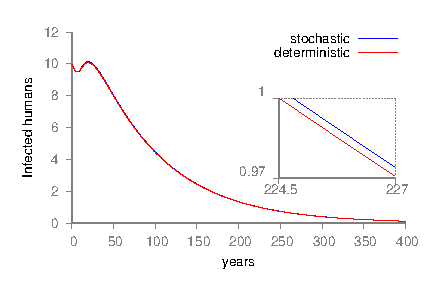
\includegraphics{%
		Sections/Section4/graphs/disease_free/disease_free_infected_humans.eps%
		}
	}
	\subfloat{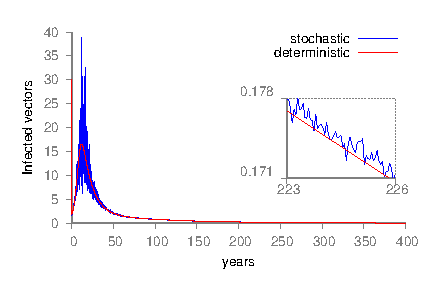
\includegraphics{%
		Sections/Section4/graphs/disease_free/disease_free_infected_vectors.eps%
		}%
	}
	\caption{}\label{Fig.1}
\end{figure}
\begin{figure}[!ht]
	\centering
	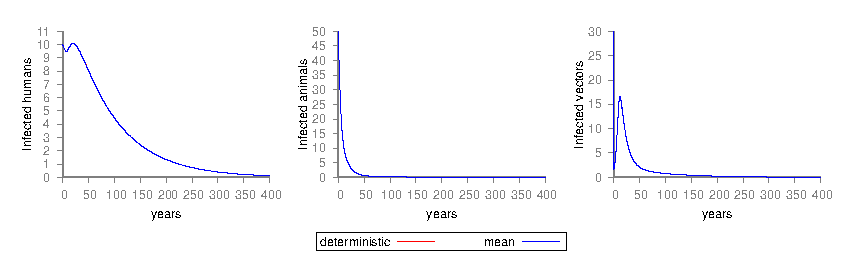
\includegraphics{%
		Sections/Section4/graphs/disease_free/disease_free_mean_population.eps%
		}%
	\caption{}\label{Fig.2}
\end{figure}
\begin{figure}[!ht]
	\centering
	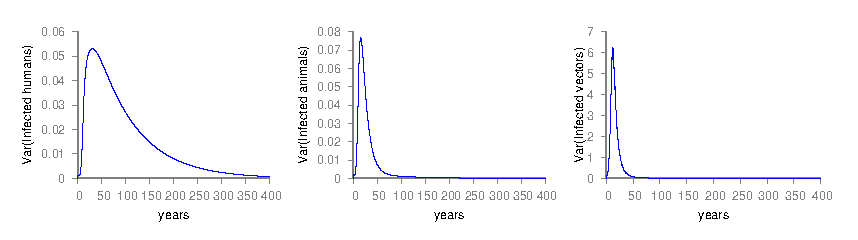
\includegraphics{%
		Sections/Section4/graphs/disease_free/disease_free_variance_population.eps%
	}
\caption{}\label{Fig.3}
\end{figure}
\todo{parameters for moment calculations}

%\begin{figure}[!ht]
%	\centering
%	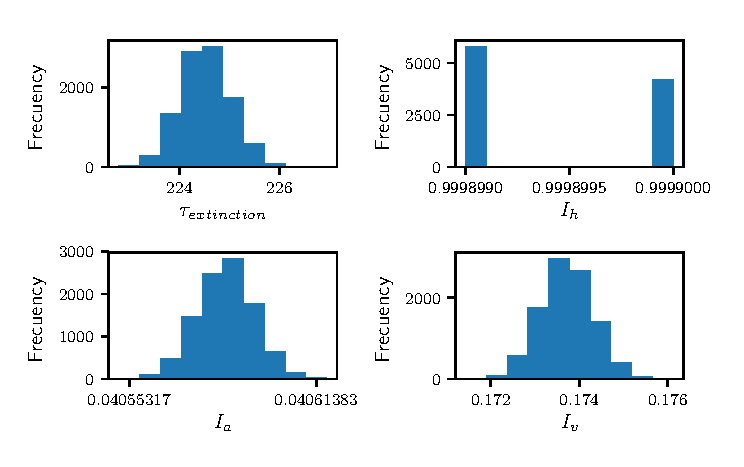
\includegraphics{%
%		Sections/Section4/graphs/disease_free/stopping_time_histograms.eps%
%	}
%\caption{}\label{Fig.3}
%\end{figure}




\subsection{Persistence}
	For guarantee the conditions of \Cref{theo:persist}, we vary the value of 
almost all parameters, thus the total animal population is equal to 
\num[group-separator = {,~}]{3000}, while total maximum allowable number of
 vectors is equal to \num[group-separator = {,~}]{12000}.
On the other hand, for this case, we consider that mortality rate for vectors 
is equal to \num{2.4455} \cite{Rabinovich1972}. The other values are given in 
\Cref{table:3}, while the parameter values that not mentioned are equal that 
in the above case.
>>>>>>> Stashed changes
%
\begin{table}[p]
	\centering
<<<<<<< Updated upstream
	\begin{tabular}{@{}llcll@{}}
		\toprule
		\multicolumn{5}{c}{Set up parameters} 												\\
		\midrule
		\\
		\multicolumn{2}{c}{Initial Conditions} &&
		\multicolumn{2}{c}{Solver Parameters}													\\
		\cmidrule{1-2} \cmidrule{4-5}																	\\
		$I_h(0)=$  \num{10}		&\phantom{abc}&& $h = \num{E-4}$				\\
		$I_a(0)=$  \num{50}		&&& $h_{res}=\num{E-6}$									\\
		$S_v(0)=$  \num{1170}	&&& 																		\\
		$I_v(0)=$  \num{30}		&&& \\
		\bottomrule
	\end{tabular}
	\caption{Set up parameters.}
	\label{tbl:initial_conditions}
=======
	\caption{
			Parameter values of system~\eqref{eq.8} to show 
			persistence
	}\label{table:3}
	\begin{tabular}{@{}crl@{}}
		\toprule
		Parameters & \multicolumn{1}{c}{Value} & \multicolumn{1}{c}{Units} \\
		\midrule
			$z_{h}$ 					& 36.5		&	$\si{bite.year^{-1}.vector^{-1}}$	\\
			$z_{a}$ 					& 182.5		&	$\si{bite.year^{-1}.vector^{-1}}$	\\
			$\tilde{\pi}_{h}$ & 0.002		&	$\si{human.bite^{-1}}$						\\
			$\pi_{h}$ 				& 0.02		&	$\si{animal.bite^{-1}}$						\\
			$\tilde{\pi}_{v}$ & 0.06		&	$\si{vector.bite^{-1}}$						\\
			$\Lambda_{v}$ 		& 2.7			&	$\si{year^{-1}}$									\\
		\bottomrule
		\end{tabular}
>>>>>>> Stashed changes
\end{table}
%
		\subsection{
			Experiment 1: Extinction --- 
			Disease-Free Equilibrium Numeric
			Analysis
		} 
				Under context of \Cref{theo:GSAS}, we use some parameter values from 
literature (see \Cref{tbl:free_disease_parameters}) and tune the rest
parameters in order to satisfies our conditions of global stochastic asymptotic
stability. Thus, we consider a whole human density of $H=\num{1500}$ habitants
which sustain $A=\num{2500}$ domestic animals. The maximum allowable number of 
vectors is assumed $20$ times host population $H$.  Likewise, we assume a
human and animals lifetime of $70$ and $6$ years, respectively, which yields
the mortalities rates 
$\mu_{h} = \num{0.0142857}\ \si{year^{-1}}$ and 
$\mu_{a} = \num{0.1666666}\ \si{year^{-1}}$. 
The vector mortality is $\mu_{v}= \num{281.1}~\si{year^{-1}}$.

	In \Cref{fig:trajectories_free_desease} we contras the effect of noise
between infected population of humans and vectors. Remember that we perturb
bitting parameters, so is feasible to obtain a most notable effect over this
population. However, as \Cref{theo:GSAS} states, we recover the extinction of
disease. We confirm these observation with the mean and variance estimation. As
we see in \Cref{fig:mean_free_disease}, the expected value of the stochastic
solution practically follows our deterministic dynamics, for this reason we get
low numerical variance at long time ---~see \Cref{fig:variance_free_disease}.
We generate \num{10 000} trajectories to estimate the mean and variance
of the infected populations. In addition, we register the first time when each 
one of this realizations achieves a level less than one individual for all 
infected populations. \Cref{fig:extinction_stopping_time_histograms} shows how
the \num{10 000} concentrates between \num{220} and \num{230} \si{years} --- 
this suggest that Chagas extinguishes (with high probability) after \num{250}
years.
%
\begin{table}[p]
	\centering
	\caption{Parameters for Experiment 1 (Survival numerics)}
	\label{tbl:free_disease_parameters}
	\begin{tabular}{@{}llllc@{}}
		\toprule
		\multicolumn{4}{c}{%
			Parameters for numerical experiment 1: disease free 
			equilibrium %
			} & \multicolumn{1}{c}{Reference}
		\\
		\cmidrule{1-3}
		$H = \num{1500}  ~\si{humans}$		&
		$A = \num{2500}  ~\si{animals}$		& 
		$K = \num{80000} ~\si{vectors}$		&
		& ---
		\\
		$\mu_h=0.0142857~\si{year^{-1}}$	&$\mu_a=0.1666666 ~\si{year^{-1}}$	& 
		$\mu_v=281.1 ~\si{year^{-1}}$ 		&																		& ---
		\\
		$z_h=14.6 ~\si{bite.year^{-1}.vector^{-1}}$			&
		$z_a=40.15~\si{bite.year^{-1}.vector^{-1}}$			&
		$\pi_{a} = \num{0.0009} ~\si{animal.bite^{-1}}$	&
		&\cite{Cruz-Pacheco2012a}
		\\
		$\pi_{h} = \num{0.0009} ~\si{human.bite^{-1}}$	 	& 
		$\pi_{v_h} = \num{0.03} ~\si{vector.bite^{-1}}$		& 
		$\pi_{v_a} = \num{0.49} ~\si{vector.bite^{-1}}$		&
		& \cite{Cohen2001}
		\\
		&&$\Lambda_v=281.561 ~\si{year^{-1}}$ &&	\cite{Rabinovich1972}
		\\
		&& $T=400 ~\si{years}$&& ---
		\\
		\\
		&\multicolumn{2}{r}{
					$\sigma_{z_a} = \num{2.2}$
					\si{bite.vector^{-1}.human^{-1}.year^{-1}}
				}
		&
		\multicolumn{2}{l}{vector human}		\\
		&
		\multicolumn{2}{r}{%
			$\sigma_{z_h} = \num{2.3}$
			\si{bite.vector^{-1}.animal^{-1}.year^{-1}}
		}
		&
		\multicolumn{2}{l}{and vector}			\\
		&
		&& 
		\multicolumn{2}{l}{animal biting}	\\
		&
		&
		&
		\multicolumn{2}{l}{intensity}\\
		&&&
		\multicolumn{2}{l}{noise}\\
		\bottomrule
	\end{tabular}
\end{table}
%
\begin{figure}[p]
	\centering
	\subfloat[][
		Extinction of the stochastic infected human %
		population.%
		]%
	{
		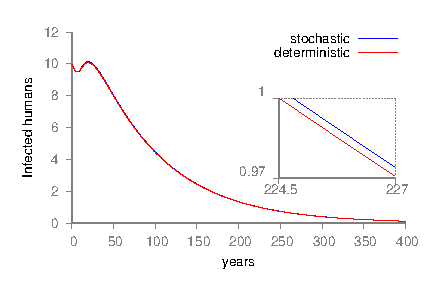
\includegraphics{%
			Sections/Section4/graphs/disease_free/disease_free_infected_humans.eps%
		}
	}
	\subfloat[][%
		Stochstic infected vector population.%
		]{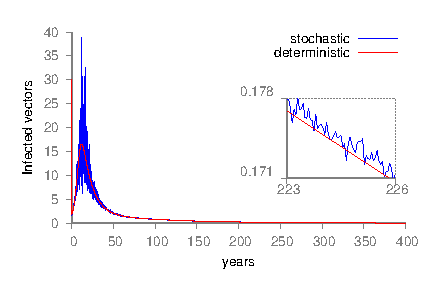
\includegraphics{%
		Sections/Section4/graphs/disease_free/disease_free_infected_vectors.eps%
	}%
	}
	\caption{
		A realization of the stochastic process solution under hypothesis of
		\Cref{theo:GSAS} for $t\in[0,400]~\si{years}$, see
		\Cref{tbl:initial_conditions,tbl:free_disease_parameters}
		for initial conditions and parameters values.
	}
	\label{fig:trajectories_free_desease}
\end{figure}
%%%%%%%%%%%%%%%%%%%%%%%%%%%%%%%%%%%%%%%%%%%%%%%%%%%%%%%%%%%%%%%%%%%%%%%%%%%%%%%%
%	Free disease moments
%
%
%%%%%%%%%%%%%%%%%%%%%%%%%%%%%%%%%%%%%%%%%%%%%%%%%%%%%%%%%%%%%%%%%%%%%%%%%%%%%%%%
\begin{figure}[p]
	\centering
	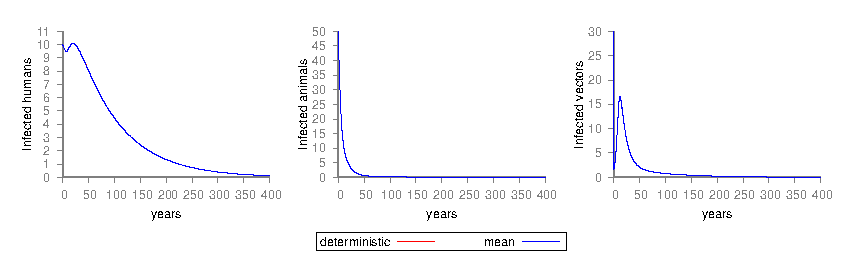
\includegraphics{%
		Sections/Section4/graphs/disease_free/disease_free_mean_population.eps%
		}%
	\caption{
		Numerical mean of \num{10000} solution trajectories
		under conditions of \Cref{theo:GSAS}.
	}
	\label{fig:mean_free_disease}
\end{figure}

\begin{figure}[p]
	\centering
	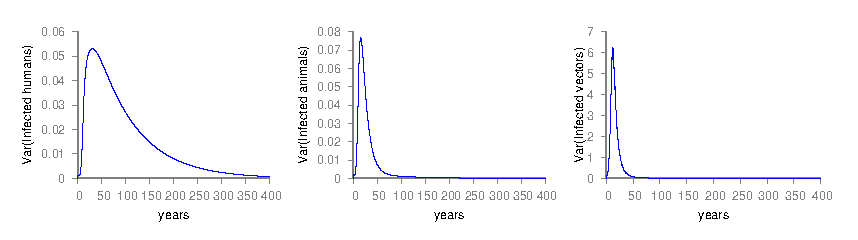
\includegraphics{%
		Sections/Section4/graphs/disease_free/disease_free_variance_population.eps%
	}
	\caption{
		Variance of \num{10000} solution trajectories under conditions of 
		\Cref{theo:GSAS}.
	}\label{fig:variance_free_disease}
\end{figure}
%%%%%%%%%%%%%%%%%%%%%%%%%%%%%%%%%%%%%%%%%%%%%%%%%%%%%%%%%%%%%%%%%%%%%%%%%%%%%%%%
%	Free disease exit time Histograms
%
%
%%%%%%%%%%%%%%%%%%%%%%%%%%%%%%%%%%%%%%%%%%%%%%%%%%%%%%%%%%%%%%%%%%%%%%%%%%%%%%%%
\begin{figure}[p]
	\centering
	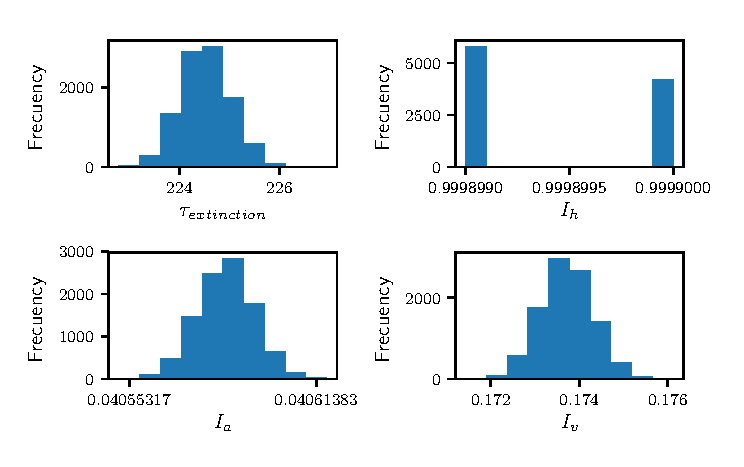
\includegraphics{%
		Sections/Section4/graphs/disease_free/stopping_time_histograms.eps%
	}
	\caption{
		Histograms of \num{10 000} sample paths under sufficient conditions for
		disease extinction see \Cref{theo:GSAS}
		and \Cref{tbl:free_disease_parameters}. As we  see at upper left, the 
		first time when all population are less than one $\tau_{extinction}$ 
		distributes its \num{10 000} occurrences around \num{220} and \num{230} 
		\si{years}.
	}\label{fig:extinction_stopping_time_histograms}
\end{figure}
		\subsection{Experiment 2: Persistence 
		--- Illness Subservience}
				Now we illustrate that Chagas survive under hypothesis of 
	\Cref{theo:persist}. For guarantee these conditions, we use the 
	paramters 
	values  of \Cref{tbl:persistence_parameters}. 
	Here, we chose the step size 
	and initial conditions from \Cref{tbl:initial_conditions}.
	In \Cref{fig:persistence_path}, we show  a sample path solution of 
	SDE \eqref{eq.8}, as we see, our stochastic extension similarly 
	follows the deterministic dynamics of \eqref{eq.1}. To confirm this claim, 
	we generate \num{10 000} trajectories to estimate statistic of the 
	solution process to SDE \eqref{eq.8}. 
	\Cref{fig:mean_persistence} shows the mean value. The histograms of 
	\Cref{fig:persistence_histograms} suggest that almost all individuals became
	infected. Finally in \Cref{fig:noise_variance_reduction} we show how
	conforming decrease the variance solutions 
	respect to the noise intensities 
	$\eta_i:=(\sigma_{z_h}^i ,\sigma_{z_a}^i)$.
	\begin{table}[p]
	\centering
	\caption{Parameters for Experiment2 (Persistence numerics)}
	\label{tbl:persistence_parameters}
	\begin{tabular}{@{}lllllc@{}}
		\toprule
		\multicolumn{4}{c}{%
			Parameters for numerical experiment 2: Persistence of the disease %
			} & \multicolumn{2}{c}{Reference}
		\\
		\cmidrule{1-4}
		$H=\num{1500} ~\si{humans}$	&&	$A=\num{3000} ~\si{animals}$	& 
		$K=\num{12000} ~\si{vectors}$&
		& ---
		\\
		$\mu_h=\num{0.0142857}~\si{year^{-1}}$	&&$\mu_a=0.1666666 
		~\si{year^{-1}}$	
		& $\pi_{a} = \num{0.02} ~\si{animal.bite^{-1}}$
		&																		& ---
		\\
		$\pi_{h} = \num{0.002} ~\si{human.bite^{-1}}$		&&
		$\pi_{v_h} = \num{0.03} ~\si{vector.bite^{-1}}$	&
		$\Lambda_v = 2.7 ~\si{year^{-1}}$
		&& ---%\cite{Cruz-Pacheco2012a}
		\\
			$T=200 ~\si{years}$&&
			$z_a = 182.5~\si{bite.year^{-1}.vector^{-1}}$		&
			$z_h = 36.5 ~\si{bite.year^{-1}.vector^{-1}}$&&	---
		\\
		&&& $\pi_{v_a} = \num{0.06} ~\si{vector.bite^{-1}}$ &&	\cite{Cohen2001}
		\\
		&&& $\mu_v=2.4455 ~\si{year^{-1}}$ && \cite{Rabinovich1972}
		\\
		\multicolumn{1}{c}{
			\Cref{fig:persistence_path,fig:mean_persistence}
		}
		&&
		\multicolumn{1}{c}{
			\Cref{fig:noise_variance_reduction}
		}
		&&
		\\
		\cmidrule{1-1}
		\cmidrule{3-3}
		&&&&
		\multicolumn{2}{l}{vector human}		\\
		\multicolumn{1}{r}{%
			$\sigma_{z_h} = \num{0.00395}$
			}
		&&
		\multicolumn{1}{l}{%
			$\sigma_{z_h}^1 = \num{.00395}$, \quad
			$\sigma_{z_h}^2 = \num{.002}$%
			
		}
		&
		\si{bite.vector^{-1}.human^{-1}.year^{-1}}
		&
		\multicolumn{2}{l}{and vector}
		\\
		\multicolumn{1}{r}{
			$\sigma_{z_a} = \num{0.00195}$
		}
		&&
		\multicolumn{1}{l}{
			$\sigma_{z_a}^1 = \num{0.00195}$, \quad
			$\sigma_{z_a}^2 = \num{0.001}$%
		}
		&
		\si{bite.vector^{-1}.animal^{-1}.year^{-1}}
		&
		\multicolumn{2}{l}{animal biting}\\
		&&&&
		\multicolumn{2}{l}{amplitude}\\
		&&&&
		\multicolumn{2}{l}{noise}\\
		\bottomrule
	\end{tabular}
\end{table}
\todo{Tabla4 $\pi_{v_h}$ unico de referencia ref[17]}
\todo{$\mu_v$ poner ref 17}


\begin{figure}[p]
	\centering
	\subfloat[][
		Stochstic sample path of infected humans
		under conditions of \Cref{theo:persist}. We made a zoom to enphasize 
		the stochastic perturbation.
	]{%
		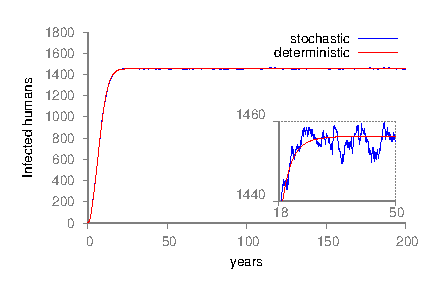
\includegraphics{%
			Sections/Section4/graphs/persistence/persistence_infected_humans.eps%
		}
	}
	\subfloat[][%
		Sotchastic bheavior of a infected animal 
		path.
		]%
	{%
		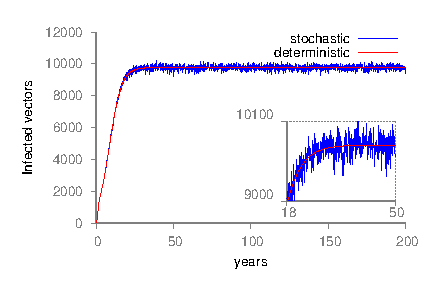
\includegraphics{%
			Sections/Section4/graphs/persistence/persistence_infected_vectors.eps%
		}
	}
	\caption{
		A sample path of the stochastic solution process
		of SDE \eqref{eq.8} under conditions of \Cref{theo:persist}.
	Parameters values in 
	\Cref{tbl:persistence_parameters}.
	}\label{fig:persistence_path}
\end{figure}

\begin{figure}[p]
	\centering
	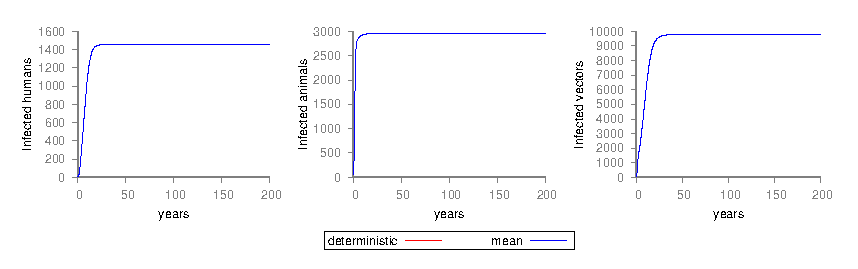
\includegraphics{%
		Sections/Section4/graphs/persistence/persistence_mean_population.eps%
	}
	\caption{
		Likening between deterministic solution and the mean of \num{10 000} 
		realizations of the stochastic solution process. As we see, our mean value 
		follows the deterministic profile.
	}
	\label{fig:mean_persistence}
\end{figure}
%%%%%%%%%%%%%%%%%%%%%%%%%%%%%%%%%%%%%%%%%%%%%%%%%%%%%%%%%%%%%%%%%%%%%%%%%%%%%%%%
%
%   Persistence Histograms at t = 200
%%%%%%%%%%%%%%%%%%%%%%%%%%%%%%%%%%%%%%%%%%%%%%%%%%%%%%%%%%%%%%%%%%%%%%%%%%%%%%%%
\begin{figure}[p]
	\centering
	\includegraphics{%
		Sections/Section4/graphs/persistence/persistence_histograms%
	}
	\caption{
		Histograms of \num{10 000} sample solution paths of SDE 
		\eqref{eq.8} under hypothesis of \Cref{theo:persist}
		and at fixed time $t=\num{200} ~\si{years}$.
	}
	\label{fig:persistence_histograms}
\end{figure}
%%%%%%%%%%%%%%%%%%%%%%%%%%%%%%%%%%%%%%%%%%%%%%%%%%%%%%%%%%%%%%%%%%%%%%%%%%%%%%%%
% Variance reduction.
%
%%%%%%%%%%%%%%%%%%%%%%%%%%%%%%%%%%%%%%%%%%%%%%%%%%%%%%%%%%%%%%%%%%%%%%%%%%%%%%%%
\begin{figure}[p]
	\centering
	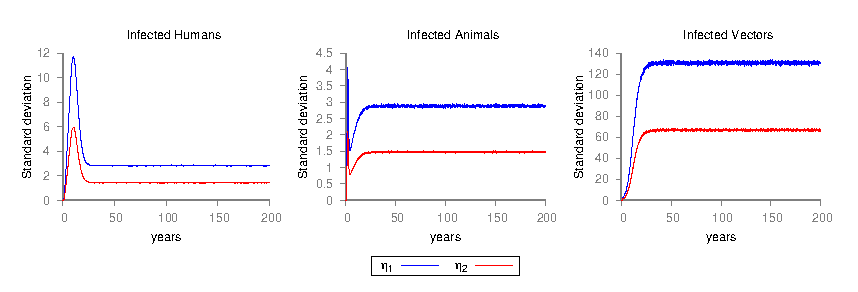
\includegraphics{%
		Sections/Section4/graphs/persistence/persistence_variance_population.eps%
	}
	\caption{
		The noise effect amplitude over variance. 
		of \num{10000} sample paths. Here we decrease the initial noise 
		intensities 
		$
			\eta_{1}:= 
			(
				\sigma_{z_h}^1,
				\sigma_{z_a}^1
			)
			=
			(
				\num{0.00395}, %~\si{bite.vector^{-1}.human^{-1}.year^{-1}}, 
				\num{0.00195} %~\si{bite.vector^{-1}.animal^{-1}.year^{-1}}
			)
		$ 
		until
		$
		\eta_{2}:= 
		(
			\sigma_{z_h}^2,
			\sigma_{z_a}^2
		)
		=
		(
			\num{0.002}, 
			%~\si{bite.vector^{-1}.human^{-1}.year^{-1}},
			\num{0.001}  
			%~\si{bite.vector^{-1}.animal^{-1}.year^{-1}}
		)
		$. As we see, this figure suggest that 
		noise intensity can modulates the solution 
		variance of SDE \eqref{eq.8}.
	}\label{fig:noise_variance_reduction}
\end{figure}
	\section{Conclusions and final comments}
			\paragraph{Future works}
As we know, in the disease modeling, there are many manner to consider the 
infection forces. Hence, we believe that generalize this characteristic will 
help to complete the present study, which we leave as future work.
		
%%%%%%%%%%%%%%%%%%%%%%%%%%%%%%%%%%%%%%%%%%%%%%%%%%%%%
	\pagebreak
	\appendix
	\renewcommand*{\thesection}{\appendixname~\Alph{section}}
	\renewcommand{\thetheorem}{\Alph{section}.\arabic{theorem}}
	\renewcommand{\thedefinition}{\Alph{section}.\arabic{definition}}
		\section{Existence and Regularity of Solutions}\label{appe.1}
	Consider the following SDE,
\begin{equation}\label{eq.ap.1}
	\begin{aligned}
		dX(t) &= f(t,X)dt + g(t,X)dW(t), \\ 
		X(t_0) &=x_0, \quad
		t\in [t_0,T].
	\end{aligned}
\end{equation}
with a non random initial condition 
$X(t_{0})=x_{0}$,
finite 
$
	T
$, 
and real coefficients
$
	f:
	\left[ 
		t_{0}, T
	\right]
	\times 
	\mathbb{R}^{d} 
	\to \mathbb{R}^{d}
$
,
$
	g:	
	\left[ 
		t_{0},T
	\right]
	\times
	\mathbb{R}^{d} 
	\to 
	\mathbb{R}^{d\times m}
$,
driven by $m$ independent standard one-dimensional Wiener processes
$W_j$, defined on a complete and filtered 
probability space
$
	\left(
		\Omega, \calF , (\calF_t)_{0\leq t\leq T},\P
	\right)
$.
We say that \Cref{eq.ap.1} has unique solution up to equivalence if for any
two solutions $X_{1}(t)$ and $X_{2}(t)$ 
$
			\mathbb{P}
			\{
				X_{1}(t)=X_{2}(t)\mbox{ for all } t \in [t_{0},T]
			\}=1
		$.

	Let $\calL$ denotes the infinitesimal generator associated to the stochastic 
	SDE~\eqref{eq.ap.1}, and defined by
\begin{equation}\label{eq.ap.2}
	\mathcal{L} =
		\frac{\partial }{\partial t} 
		+
		\sum_{i=1}^d
			f_{i}(t,X(t))
			\frac{\partial}{\partial x_{i}}
			+
			\frac{1}{2}
		\sum_{i,j=1}^m
			\left(
				g(t, X(t)) g^{T}(t, X(t))
			\right)_{ij}
			\frac{\partial^{2}}{\partial x_{i}\partial x_{j}}.
\end{equation}
Under the above, we use a part of the result for existence and unique of 
solutions enunciated by \citeauthor*{Khasminskii2012} in \cite{Khasminskii2012}.
\begin{theorem}[{\citet[Theorem 3.4]{Khasminskii2012}}]\label{thm:existence}
	Let the vectors 
	$$
		f(t,x), \quad g_1(t,x), ..., g_m(t,x), \quad
		t\in [t_{0},T],
		\qquad x\in \R^{d},
	$$
	be continuous functions of $(t,x)$, such that for some constant $B$ the 
	following conditions hold in the entire domain of definition:
	\begin{equation}
		\begin{aligned}\label{eq.ap.3}
			\norm{
				f(t,x)- f(t,y)
			} 
			&+ 
			\sum
				\limits_{r=1}^{m}
				\norm{
					g_{r}(t,x)- g_r(t,y)
				}
			\leq B 
			\norm{x-y},\\
			\norm{
				f(t,x)} 
				&+ 
				\sum
				\limits_{r=1}^{m}
				\norm{
					g_r(t,x)} 
				\leq B (1 + \norm{x}) ~.
		\end{aligned}
	\end{equation}
	Then, for every random variable $X(t_{0})$ independent of the process 
	$W_{r}(t)-W_{r}(t_{0})$ there exists a solution $X(t)$ of~\eqref{eq.ap.1} 
	which is almost surely continuous stochastic process and is unique up to 
	equivalence.
\end{theorem}
Also, we applied the following result in order to assure regularity of 
solutions to our SDE model.
\begin{theorem}[{\citet[Corollary 3.1]{Khasminskii2012}}]\label{theo.ap.2}
	Let $\mathsf{D}$ and $\mathsf{D}_{n}$, for each positive integer $n$, be open 
	sets in $\mathbb{R}^{d}$, such that
	\begin{eqnarray*}
		\mathsf{D}_{n}
		\subseteq 
		\mathsf{D}_{n+1},
		\ \ \overline{\mathsf{D}}_{n}
		\subseteq \mathsf{D},
		\ \ \mbox{and}
		\ \ \mathsf{D}
		=\displaystyle \bigcup_{n}{\mathsf{D}_{n}},
	\end{eqnarray*}
	Suppose that in every cylinder $[ t_{0},\infty)\times \mathsf{D}_{n}$, the 
	functions $f(t,x)$ and $g_r(t,x)$ satisfy conditions~\eqref{eq.ap.3} 
	and there exists a function $V(t,x)$, twice continuously differentiable in 
	$x$ and continuously differentiable in $t$ in the domain 
	$[ t_{0},\infty)\times \mathsf{D}$, such that for some positive constant $c$
	it holds that $\mathcal{L}V\leq cV$ and,
	\begin{eqnarray*}
		\inf_{t\geq t_{0}, 
		x \in \mathsf{D}
		\backslash 
		\mathsf{D}_{n}} 
		V(t,x)\to \infty ,
		\ \ \ \ \text{ as }
		\ \ n \to \infty,
	\end{eqnarray*}
	then, the conclusion of \Cref{thm:existence} holds provided that also 
$\mathbb{P}(x(t_{0})\in \mathsf{D})=1$. Moreover, the solution satisfies that 
$$
	\mathbb{P}(x(t)\in \mathsf{D})=1,\mbox{ for all }t\geq t_{0} ~.
$$
\end{theorem}
\section{Stability}\label{appe.2}
	\begin{definition}
		We say that $x^{*}$ is an equilibrium position of the SDE·\eqref{eq.ap.1} 
		if $f(t,x^{*})=0$ and $g(t,x^{*})=0$ for all
	$t\geq t_{0}$.
\end{definition}
%
\begin{definition}[{\citet[Section 5]{Khasminskii2012}}]\label{dfn:app3}
	Let $x^{*}$ as above definition and
	$
		X^{t_{0},x_{0}}
	$
	the solution of \eqref{eq.ap.1} whit initial condition $X(t_0)=x_0$.
	\begin{enumerate}[(i)]
		\item The equilibrium solution $x^{*}$ of equation~\eqref{eq.ap.1} is said 
		to be stable in probability for $t\geq 0$ if for any $t_{0}\geq 0$ and 
		$\epsilon >0$
		\begin{align*}
			\lim\limits_{x_{0}\rightarrow x^{*}}\mathbb{P}
			\left\lbrace 
				\sup\limits_{t>t_{0}} 
				\norm{X^{t_{0},x_{0}}-x^{*}}> \epsilon 
			\right\rbrace = 0.
		\end{align*}
		\item 
			The equilibrium solution $x^{*}$ is said to be asymptotically 
			stable in probability if it is stable in probability and 
			\begin{align*}
			\lim\limits_{x_{0}
				\rightarrow x^{*}}\mathbb{P}
				\left\lbrace 
					\lim\limits_{t\rightarrow \infty}X^{t_{0},x_{0}}(t)=x^{*}
				\right\rbrace = 1.
			\end{align*}
		\item
			The equilibrium solution $x^{*}$ is said to be (asymptotically) 
			stable in the large if it is stable in probability and also for all 
			$t_{0},x_{0}$
			\begin{align*}
				\mathbb{P}
					\left\lbrace 
						\lim
						\limits_{t\rightarrow \infty}X^{t_{0},x_{0}}(t)=x^{*}
					\right\rbrace =1.
			\end{align*}
	\end{enumerate}
\end{definition}
%
\begin{definition}[{\citet[p. 108]{Mao2007}}]\label{dfn:radial_unbonded}
	A function $V(x,t)$ defined on 
	$\mathbb{R}^{d}\times\left[t_{0},\infty\right)$ is said to be radially 
	unbounded if
	\begin{align*}\label{def.radi}
		\lim
		\limits_{\norm{x}\rightarrow\infty}
		\inf\limits_{t\geq t_{0}}V(x,t)=\infty.
	\end{align*}
\end{definition}
%
\begin{theorem}[{\citet[Theorem 2.4]{Mao2007}}]\label{theo.ap.3}
	Suppose that the assumptions of \Cref{thm:existence} holds for
	$t\geq t_{0}$, and let 
	$S_{h} = 
		\{ 
			X\in \R^{d}:
			\norm{X-x^{*}}<h
		\}
	$. 
	If there exists a positive-definite decrescent radially unbounded 
	function 
	$
		V(x,t)\in C^{2,1}
		\left(
			S_{h}\times \left[t_{0},\infty 
		\right);
		\mathbb{R}_{+}\right)
	$, such that $\mathcal{L}V(x,t)$ is 
	negative-definite, 
	then the equilibrium solution $x^{*}$ of 
	equation~\eqref{eq.ap.1} is stochastically asymptotically stable in the large.
\end{theorem}
%
\begin{lemma}[%
		Strong Law of Large Numbers for Martingales %
		{\citep[Theorem 3.4]{Mao2007}}
	]\label{lem.marting}
	Let $Μ = \left\{M_t\right\}_{t \geq 0}$ be a real--valued continuous local 
	martingale vanishing at $t = 0$. 
	If $M$ has finite quadratic variation, then
	$$
		\lim_{t \to \infty} \frac{M_t}{t}=0.
	$$
\end{lemma}
\section{Linear-Steklov Method}\label{app:ls_method}
		According to SDE \eqref{eq.2}, let 
%
\begin{equation*} \label{eqn:SDE_coefficients}
	\begin{aligned}
			y(t)&:=(I_h(t),I_a(t),S_v(t),I_v(t))^T,
			&&
			F_{1} = 
				F_{1}
					\left(
						I_{h}(t),I_{a}(t),S_{v}(t),I_{v}(t)
					\right),
			\\
			F_{2} &=
				F_{2}
					\left(
						I_{h}(t),I_{a}(t),S_{v}(t),I_{v}(t)
					\right)
			\\
			f(y) &:= 
			\begin{bmatrix} 
				\alpha_{h}I_{v}\left(H-I_{h}\right)-\mu_{h}I_{h} \\
				\alpha_{a}I_{v}\left(A-I_{a}\right)-\mu_{a}I_{a} \\
				\Lambda_{v}T_{v}
				-\left(
					\alpha_{v_{h}}I_{h}
					+\alpha_{v_{a}} I_{a}
				\right)S_{v}
				-\left(
					\mu_{v}+r_{K}T_{v}
				\right)S_{v}\\
				\left(
					\alpha_{v_{h}}I_{h}+\alpha_{v_{a}}I_{a}
				\right)
				S_{v}
				-\left(
					\mu_{v}+r_{K}T_{v}
				\right)I_{v}
			\end{bmatrix}, 
			&&
			g(y):=
			\begin{bmatrix}
				F_{1}\theta_{h}I_{v}\left(H-I_{h}\right) & 0 \\
				0 & F_{2}\theta_{a}I_{v}\left(A-I_{a}\right) \\
				- F_{1}\theta_{v_{h}}I_{h}S_{v} & -F_{2}\theta_{v_{a}}I_{a}S_{v} \\
				F_{1}\theta_{v_{h}}I_{h}S_{v} & F_{2}\theta_{v_{a}}I_{a}S_{v} \\
			\end{bmatrix}.
	\end{aligned}
\end{equation*}
	Following the notation of \cite{Diaz-Infante2016} and 
after some manipulations, we rewrite each drift
component  function $f^{(j)}:\R^4:\to \R$, 
$j \in \{1,\dots, 4\}$ of SDE \eqref{eq.8} as
\begin{equation*}\label{eqn:AlternativeConstruction}
	f^{(j)}(y) = a_j (y) y^{(j)} + b_{j}(y^{(-j)}), \qquad
	y^{(-j)} = 
		(y^{(1)}, 
			\dots , y^{(j-1)}, y^{(j+1)}, 
			\dots, y^{(d)}
		)^T,
\end{equation*}
where
\begin{align*}
	a_1(y)&:=
		-\left(
			\alpha_{h} y^{(4)} +\mu_{h}
		\right),
	&
	b_1(y)&:= 
		\alpha_h  y^{(4)} H ,
	\\
	%
	a_2(y) &:=
		-
		\left(
			\alpha_{a} y^{(4)}+\mu_{a}
		\right),
	&
	b_2(y)&:= 
		\alpha_a  y^{(4)} A ,
	\\
	a_3(y) &:=
		-
		\left( 
			 \alpha_{v_{h}} y^{(1)}
			+ \alpha_{v_{a}} y^{(2)}
			+ r_K (y^{(3)} + y^{(4)})
			+\mu_v
			- \Lambda_v
		\right),
	&
	b_3(y)&:= 
		\Lambda_{v} y^{(4)},
		\\
	a_4(y) &:=
		-
		\left(
			\mu_{v}
			+r_k
			\left(
				y^{(3)} + y^{(4)}
			\right)
		\right),
		&
	b_4(y) &:=
		\left(
			\alpha_{v_h} y^{(1)}
			+
			\alpha_{v_{a}} y^{(2)}
		\right)
		y^{(3)} ~.
\end{align*}
Let $h$ the step size. Consider the matrices 
$
	A^{(1)}= A^{(1)}(h,y)
$,
$
A^{(2)}= A^{(2)}(h,y)
$
defined by
\begin{align*}
	A^{(1)}&:=
		\begin{pmatrix}
			e^{ha_1(y)} & 
			\multicolumn{2}{c}{
				\text{\kern0.5em\smash{\raisebox{-1ex}{\huge 0}}}
			} \\
			&\ddots\\
			\multicolumn{2}{c}{
				\text{\kern-0.5em\smash{\raisebox{0.95ex}{\huge 0}}}} 
			& e^{ha_4(y)}
		\end{pmatrix}, \notag
		\\
%
	A^{(2)}&:=
		\begin{pmatrix}
			\left(
				\displaystyle
				\frac{e^{ha_1(y)} - 1}{a_1(y)}
			\right)\1{E_1^c}
			& 
			\multicolumn{2}{c}{\text{\kern0.5em\smash{\raisebox{-1ex}{\huge 0}}}}\\
			& \ddots&\\
				\multicolumn{2}{c}{\text{\kern0.5em\smash{\raisebox{-1ex}{\huge 0}}}}&
			\left(
				\displaystyle
				\frac{e^{h a_4(y)} - 1}{a_4(y)}
			\right)\1{E_4^c}
		\end{pmatrix}
		+h
		\begin{pmatrix}
			\1{E_1} 
			&
			\multicolumn{2}{c}{\text{\kern0.5em\smash{\raisebox{-1ex}{\huge 0}}}}\\
			&
			\ddots 
			&\\
			\multicolumn{2}{c}{\text{\kern0.5em\smash{\raisebox{-1ex}{\huge 0}}}} 
			&\1{E_4}
		\end{pmatrix},\\
		E_j&:=\{y \in \R^4: a_j(y)=0\} , \qquad 
		b(y):= 
			\left(
				b_1(y^{(-1)}), \dots , b_4(y^{(-4)})
			\right)^T.
		\notag
\end{align*}
Thus, given $Y_0=y(0)$, and $h = T/N$, the LS method for 
SDE \eqref{eq.8} reads
\begin{equation}
	\begin{aligned}\label{eqn:LS-scheme}
		Y_{k+1} &= 
			A^{(1)}(h,Y_k)Y_k
			+ A^{(2)}(h,Y_k) b(Y_k) + g(Y_k) \Delta W_k
						,\qquad k=0,\dots, N-1.
	\end{aligned}
\end{equation}
Since \Cref{thm:regularity} ensures positivity of the SDE \eqref{eq.2} solution,
in order to preserves this property, we modify the  
scheme \eqref{eqn:LS-scheme} as
\begin{equation}
	\begin{aligned}
		Y_k^{\star} &= 
				A^{(1)}(h,Y_k)Y_k
				+ A^{(2)}(h,Y_k)b(Y_k) + g(Y_k) \Delta W_k \\
		Y_{k+1} &=
			\left(
				\1{ Y_k^{\star}\geq 0} 
				-
				\1{ Y_k^{\star} < 0}
			\right)Y_{k}^{\star} ~.
	\end{aligned}
\end{equation}
\todo{
	review if our diffusions
	satisfies dissipative conditions
}

	\section*{References}
		\bibliographystyle{model6-num-names}
		\bibliography{sde}
\end{document}